\documentclass[10pt,a4paper]{article}
\usepackage{comment}
\usepackage{geometry}
\usepackage{graphicx}
\usepackage{amsthm,amsfonts,mathrsfs}
\usepackage{enumerate}

\usepackage{amsmath,accents}
\usepackage{amsfonts}
\usepackage{amssymb}
\usepackage{relsize}
\usepackage{latexsym}
\usepackage{subfigure}
\usepackage{hyperref,cleveref}
\usepackage{nomencl}
\usepackage[dvipsnames]{xcolor}
\usepackage[normalem]{ulem}
\usepackage{bold-extra}
\usepackage{tabto}
\usepackage{tikz}
\usepackage{titlesec}
\newcommand{\eqname}[1]{\tag*{#1}}
\setcounter{secnumdepth}{4}
\titleformat{\paragraph}
{\normalfont\normalsize\bfseries}{\theparagraph}{1em}{}
\titlespacing*{\paragraph}
{0pt}{3.25ex plus 1ex minus .2ex}{1.5ex plus .2ex}
\usetikzlibrary{shapes,arrows}
\tikzstyle{decision} = [diamond, draw,
    text width=4.5em, text badly centered, node distance=3cm, inner sep=0pt]
\tikzstyle{block} = [rectangle, draw, fill=blue!20,
    text width=5em, text centered, rounded corners, minimum height=4em]
\tikzstyle{line} = [draw, -latex']
\tikzstyle{cloud} = [draw, ellipse,fill=red!20, node distance=3cm,
    minimum height=2em]
\setlength{\parindent}{0pt}
\TabPositions{5.cm}
\newcommand{\nomunit}[1]{\renewcommand{\nomentryend}{\hspace*{\fill}#1}}

\newcommand{\partder}[2]{\ensuremath{\frac{\partial #1}{\partial #2}}}
\newcommand{\secpartder}[2]{\ensuremath{\frac{\partial^2 #1}{\partial #2^2}}}
\newcommand{\nthpartder}[3]{\ensuremath{\frac{\partial^{#1}
#2}{\partial #3^{#1}}}}
\newcommand{\fullder}[2]{\ensuremath{\frac{\mbox{d} #1}{\mbox{d} #2}}}
\newcommand{\secfullder}[2]{\ensuremath{\frac{\mbox{d}^2 #1}{\mbox{d} #2^2}}}
\newcommand{\nfullder}[3]{\ensuremath{\frac{\mbox{d}^{#1} #2}{\mbox{d}
#3^{#1}}}}
\newcommand{\mixedder}[3]{\ensuremath{\frac{\partial^{2} #1}{\partial
#2 \partial #3}}}
\newcommand{\df}[1]{\, \ensuremath{\mbox{d}#1}}
\newcommand{\grad}{\, \mbox{grad} \,}
\newcommand{\dive}{\, \mbox{div} \,}
\newcommand{\real}[1]{\text{Re} \left\{ #1 \right\}}
\newcommand{\imag}[1]{\text{Im}\left\{ #1 \right\}}
\newcommand{\commentstm}[1]{\textcolor{blue}{\textbf{STM:\ #1}}}
\newcommand{\commentstmtwo}[1]{\textcolor{purple}{\textbf{STM:\ #1}}}
\newcommand{\newstm}[1]{\textcolor{red}{\textbf{#1}}}
\newcommand{\newstmtwo}[1]{\textcolor{orange}{\textbf{#1}}}
\newcommand{\oldstm}[1]{\sout{#1}}
\newcommand{\oldstmtwo}[1]{\xout{#1}}
\newcommand{\eqlabelsigi}[1]{\label{eq:#1}  \tag*{\texttt{#1}}}
\newcommand{\brok}{\textcolor{ForestGreen}{\textit{\textbf{OK for Bernhard}}}}
\newcommand{\apok}{\textcolor{ForestGreen}{\textit{\textbf{OK for Andr\'{e}}}}}
\newcommand{\brnok}{\textcolor{red}{\textit{\textbf{NOT OK for Bernhard}}}}
\newcommand{\apnok}{\textcolor{red}{\textit{\textbf{NOT OK for Andr\'{e}}}}}

\newcommand{\commentbr}[1]{\textcolor{orange}{\textbf{BR:\ #1}}}


\newcommand{\xs}{\mathbf{x}_\text{s}}
\newcommand{\xr}{\mathbf{x}_\text{r}}
\newcommand{\x}{\mathbf{x}}
\newcommand{\n}{\mathbf{n}}
\newcommand{\s}{\mathbf{s}}

\newtheorem{thm}{Theorem}[section]
\makenomenclature
%opening

\title{Full Waveform Inversion}
\author{ALTEN Netherlands\\
MELISSEN, S.T.A.G., version of November 21, 2018}

\begin{document}
\maketitle
\newpage
\tableofcontents
\newpage
\section{Preface}
This document describes a method to predict the size and shape of unexplored oil reserervoirs based on acoustic testing that ALTEN developed based on Peter Haffinger's Ph.D. thesis (TU Delft 2013).
The current version is in progress and written by S. Melissen, under the supervision of Andr\'e\ Prins and Bernhard Righolt.
It follows a pre-version by Nikita Mahto.
The development currently takes place on the ``serial''-branch of the git repository, where the parallelization and non-C++ code is being completely split out to have a comprehensible, single CPU version that works on a variety of machines in a more or less ``plug-and-play'' manner.
The Master branch functions relatively well (see ``Results'').
This branch will be split out into a development branch, where the parallelization introduced in the Master branch is cleaned up completely and clearly split out as one option upon several computational methods.
The Docs branch - where this document will be posted - is supposed to clear up documentation issues, the code being in a functioning, albeit very confusing state.

\newpage
\clearpage
\section{Introduction}

The Full Wave inversion is an advanced imaging
technique which can be achieved by
irradiating the interior of
an object with e.g. acoustic or electromagnetic
waves, while receivers placed around the object measure the response.
From these measurements an image of the properties of the object's
interior can be derived.

It has various applications including,

\begin{enumerate}
    \item seismology
    \item medical: ultrasonic applications
\end{enumerate}

Figure \ref{fig:FWI1} displays the perspective views of Axial
Volcano’s internal structure, constructed using elastic full waveform
inversion (FWI) results along seismic lines across caldera and along
the secondary magma reservoir. (a): P-wave velocity structure. (b):
Total gradient magnitude of the P-wave velocity structure. (c)
Reflectivity structure. The red mesh marks the extent of the main
magma reservoir on (a) and (b).

\begin{figure}[h!]
  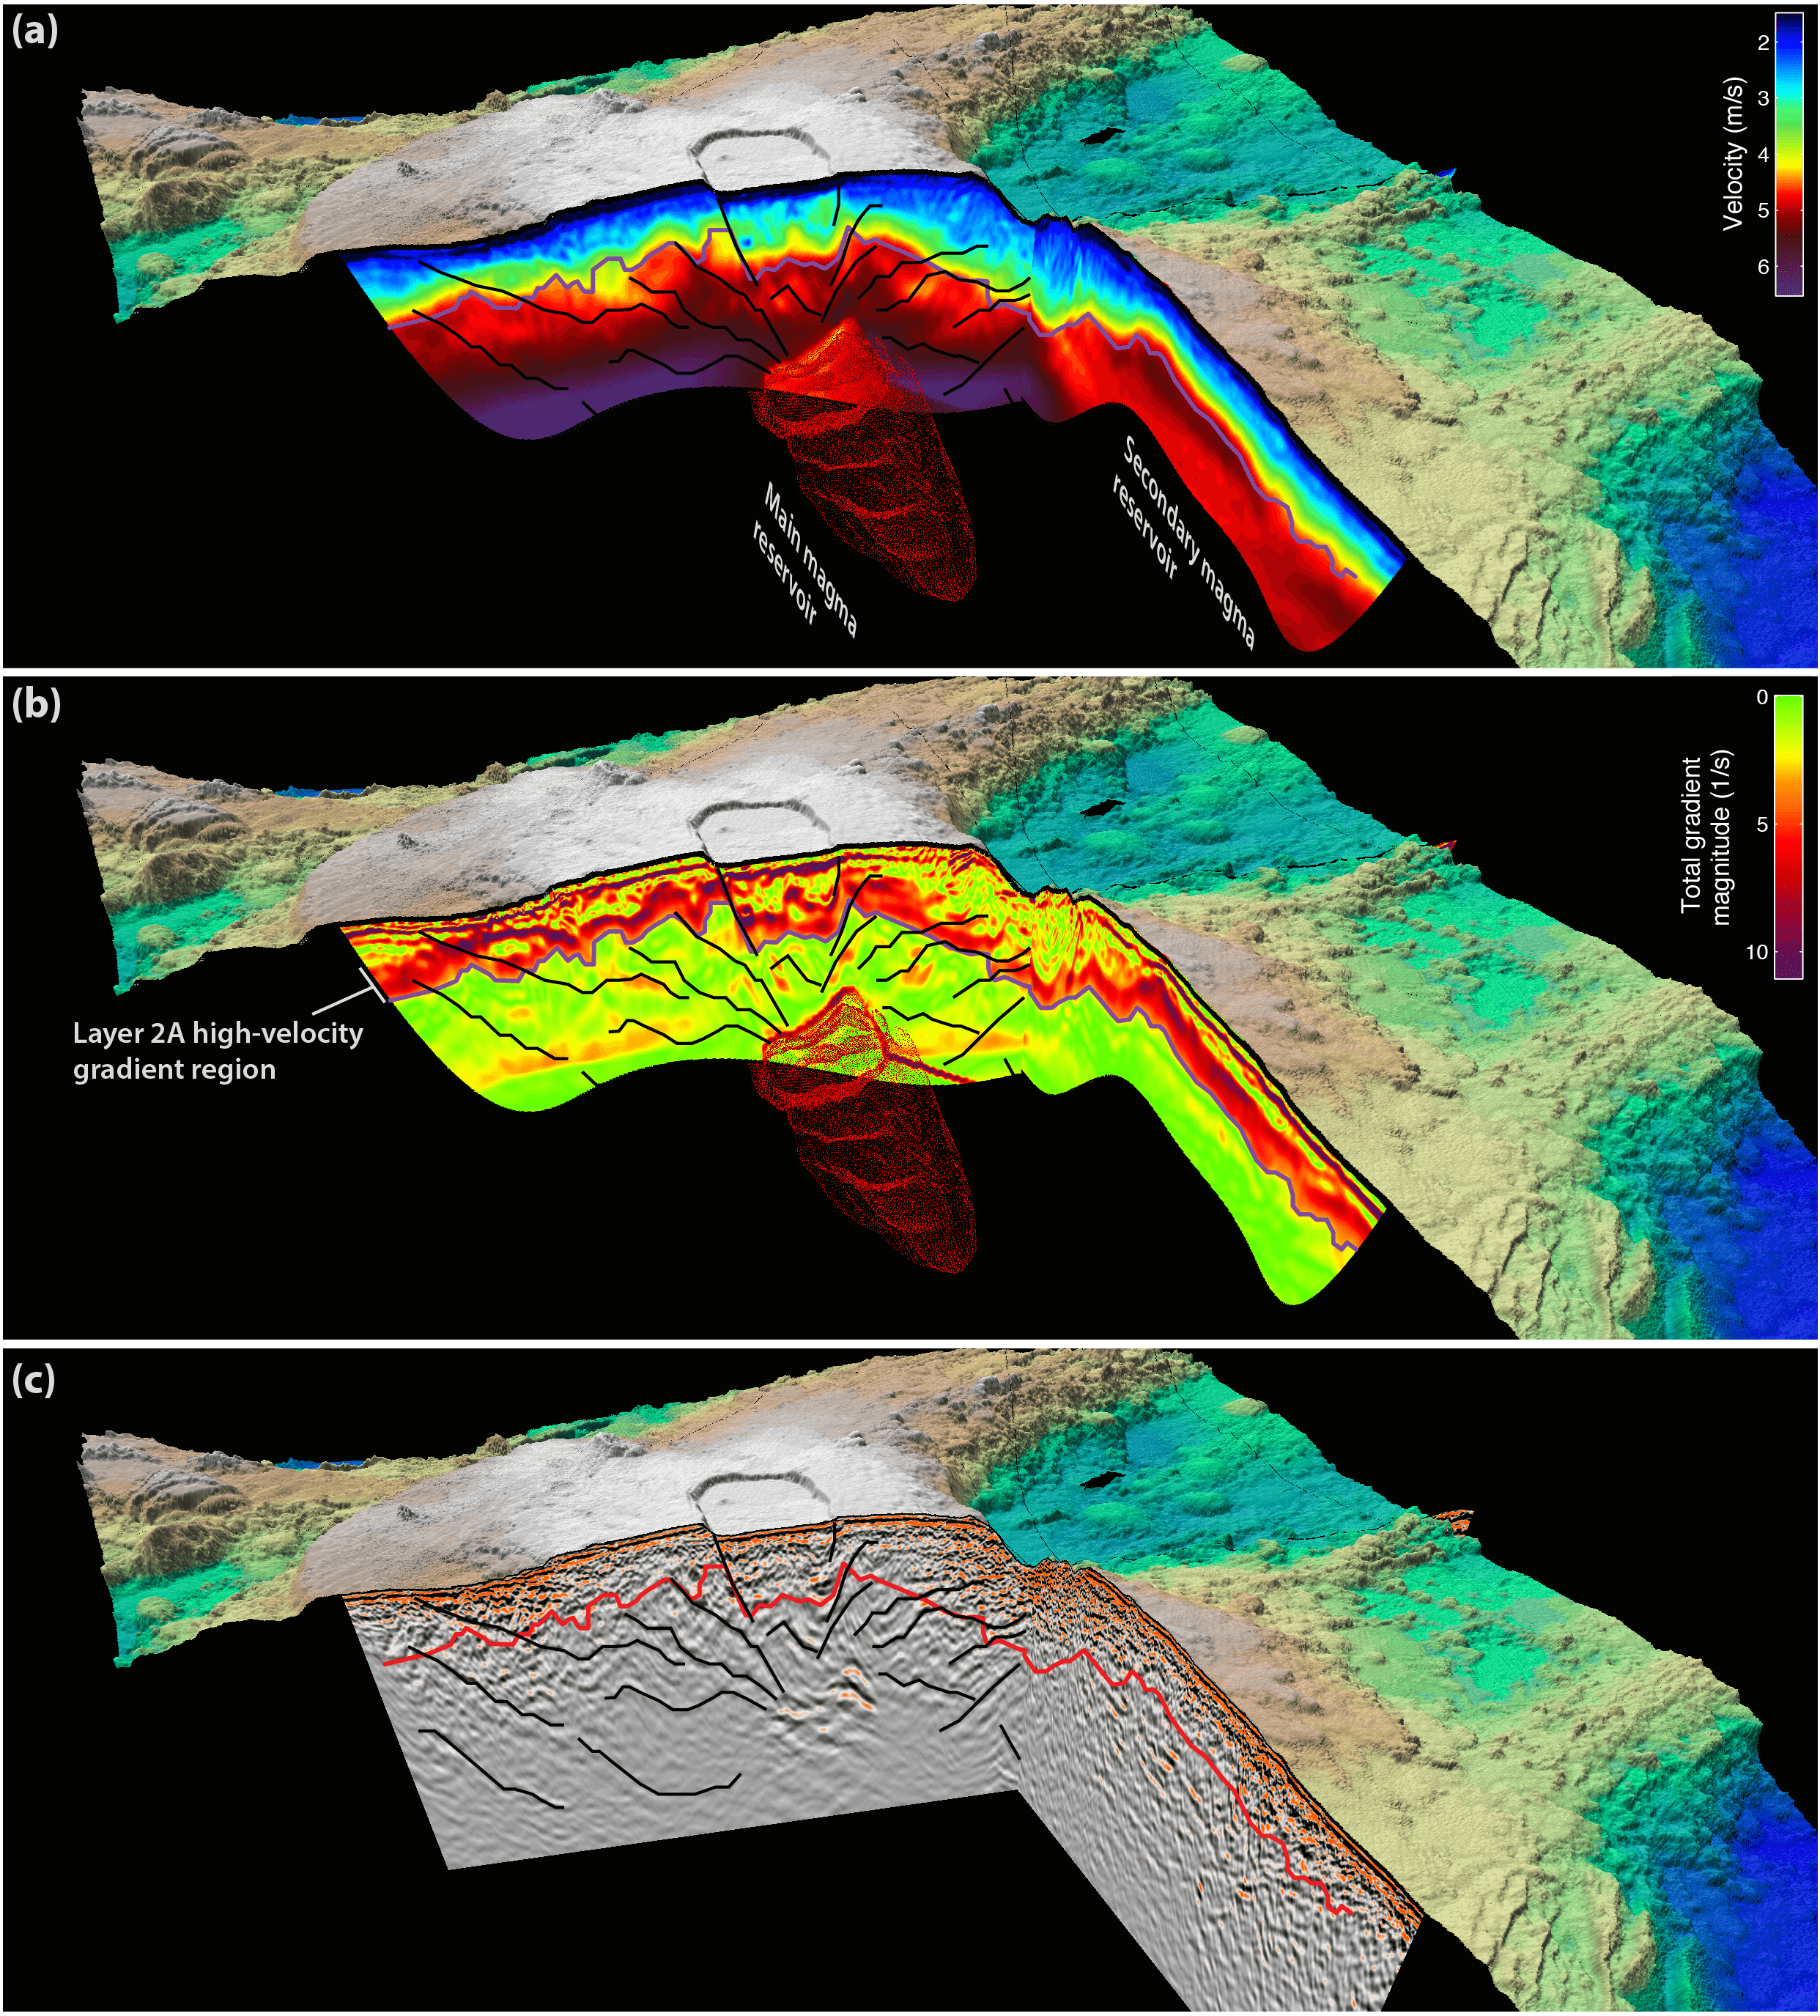
\includegraphics[width=0.75\linewidth]{FWI1.png}
  \caption{Seismic Full Waveform Inversion}
  \label{fig:FWI1}
\end{figure}

In FWI, the aim is to find the media properties on a dense subsurface grid. It is important to mention that unlike the real applications in which the recorded data by the receivers are provided, in this project only the expected image (indicating the media properties) is provided while the recorded data by the receivers (pressure field) are not available. Therefore in the first step, the recorded pressure field should be generated, knowing the expected media properties (for example, the input image of the temple) and a forward model which is explained in this report. This part has been developed in a separate \textit{preProcessing} application. After generating the recorded pressure field, the same forward model has been used to reconstruct the expected media properties (input image). First the initial estimated pressure field is initialized by an arbitrary value of media properties in the existing forward model. Afterwards, the difference between the estimated pressure field and the recorded data (objective function) are calculated. In an iterative process, the idea is to minimize this objective function (residual) by updating the unknown media property values using any optimization technique. Finally, we expect to ideally estimate the expected values of the media properties. This part is implemented in the \textit{processing} application.

Figure \ref{fig:FWI2}, shows a flowchart of the FWI project. In future, by having the access to real recorded data by the receivers, the developed \textit{preProcessing} application (orange blocks in the figure) should be replaced by just reading the measured data.

% \begin{figure}
% \centering
% \begin{tikzpicture}[node distance = 2cm, auto]
%     \node [draw,rectangle split, rectangle split horizontal,rectangle
% split parts=3] (init) {\nodepart{two}{\shortstack{Forward\\
% Modeling}}};
%     \node [draw, trapezium,trapezium left angle=70,trapezium right
% angle=-70, left of=init, node distance = 3cm, fill=green!10] (expert)
% {\shortstack{Starting\\ Model}};
%     \node [draw, trapezium,trapezium left angle=70,trapezium right
% angle=-70,right of=init, node distance = 3cm, fill=blue!20] (system)
% {\shortstack{Synthetic\\ Data}};
%     \node [draw, below of=system, rectangle split, rectangle split
% horizontal,rectangle split parts=3] (identify)
% {\nodepart{two}{\shortstack{Residual\\ Derivation \& \\ Inversion}}};
%         \node [draw, trapezium,trapezium left angle=70,trapezium right
% angle=-70,right of=identify, node distance = 3cm, fill=blue!60]
% (new){\shortstack{Real\\ Data}};
%     \node [draw, trapezium,trapezium left angle=70,trapezium right
% angle=-70,below of=identify, fill=green!55, node distance=4cm]
% (evaluate) {\shortstack{Updated\\ Model}};
%     \node [decision, left of=evaluate, fill=orange] (decide)
% {\shortstack{Con-\\ verged\\ ?}};
%     \node [decision, left of=evaluate, fill=red, below of=init, minimum width = 7 cm, align=flush left]
% (unconverged) {\shortstack{Max.\\ No. of iterations n\_max \\ reached\\ ?}};
%     \node [draw, trapezium,trapezium left angle=70,trapezium right
% angle=-70,left of=decide, node distance = 3cm, fill=green] (stop)
% {\shortstack{Final\\ Model}};
%     \path [line] (system) -- (identify);
%     \path [line] (identify) -- (evaluate);
%     \path [line] (evaluate) -- (decide);
%     \path [line] (decide) -- node {no}(unconverged);
%     \path [line] (decide) -- node {yes}(stop);
%     \path [line] (unconverged) -- node {yes}(stop);
%     \path [line] (unconverged) -- node {no}(init);
%     \path [line] (expert) -- (init);
%     \path [line] (init)|-(system);
%     \path [line] (new)--(identify);
% \end{tikzpicture}
% \caption{Full Waveform Inversion Methodology. \label{fig:FWI2}
% \commentstmtwo{Warning, the example remaining from the previous versions appears to be an unconverged temple.}}
% \end{figure}
% \begin{comment}
% \end{comment}

\begin{figure}[h!]
  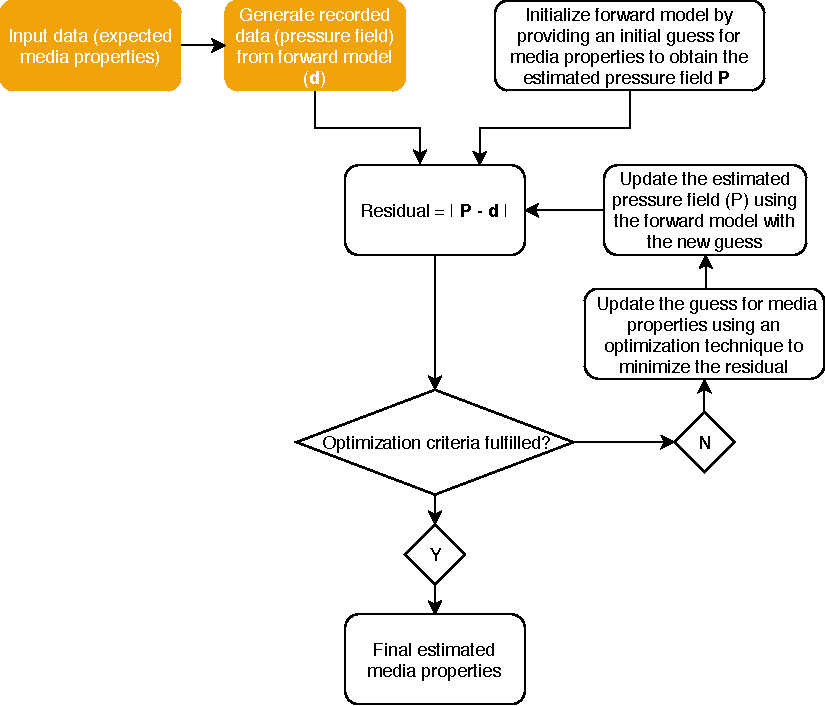
\includegraphics[width=0.75\linewidth]{FWI_crop.pdf}
  \caption{Full Waveform Inversion Methodology} 
  \label{fig:FWI2}
\end{figure}

This document provides an overview of the
equations employed, the computational model and the code algorithm.
The approach is based on the Ph.D. thesis by Peter R. HAFFINGER (TUDelft 2013) ``Seismic Broadband Full Waveform Inversion
by shot/receiver refocusing''
\section{The Model}
\subsection{Physical model}

The mathematical model outlines the equations used in the code for the FWI.
We begin with the Green's function and apply it to the
simplest acoustic equation - the Helmholtz equation.
For the acoustic case with constant density, the wave equation can be
described by two equations,
being the data equation and the object equation. The data equation
describes the seismic dataset, in terms of a total field
$p_{\text{tot}}$ at each grid point in the subsurface, the contrast
function $\chi$ and the Green's function $\mathcal{G}$
in a background medium: 

\begin{align}
\label{eq:calculateData}
p_\text{data}(\mathbf{x_\text{r}},\mathbf{x_\text{s}},\omega) = \int
\mathcal{G}(\xr, \x, \omega) p_\text{tot}(\x, \xs, \omega) \chi(\x)
\df{\x}\\
\tag*{\texttt{eq:calculateData, see include/inversion.h\footnotemark}}
\end{align}\footnotetext{``eq:'' denotes equations that are implemented in the code, ``step:'' denotes equations we present to understand the flow of this manual. Inside the code, the implementation of these equations is marked with such symbols. There, ``rel:'' means that an equation is related to the ``eq'', similar to the use of ``step'' here.}

Reading from right to left, equation \ref{eq:calculateData} can be understood as
follows: A source transmits a wavefield that propagates to every point
in the subsurface. Note that this wavefield $p_\text{tot}$ is
generally quite complex because it takes the interaction of all
scatterers in the subsurface already into account. This wavefield is
creating secondary sources in all points where the contrast function
$\chi$ is non-zero. The secondary sources transmit energy through a
smooth background medium to the receivers, represented by the Green's
function $\mathcal{G}$ in equation \ref{eq:calculateData}.\\ %\linebreak
%\newline
The measured seismic data at every receiver are then a summation of
all secondary sources. It should be mentioned that direct waves,
including ground roll and surface waves are supposed to be removed
from the measured data to obtain $p_\text{data}$.

We use the 2-D case for the Helmholtz equation. Further, the Green's
function is calculated for this equation. The contrast function has to
be determined. Further the conjugate scheme is established to
determine the error functional.

Measured seismic data always contains some form of noise, so the
inversion process is required to be regularised. Therefore, we extend
the conjugate gradient scheme so as to include a multiplicative regularisation factor.

\subsubsection{The Green's function}
A Green's function is the impulse response of an inhomogeneous linear
differential equation defined on a domain, with specified initial
conditions or boundary conditions.
The Green's function of this equation is defined as the solution
$\mathcal{G}(\mathbf{x}, \mathbf{y})$, of the equation

\begin{align}
\label{eq:GeneralGreensFunc}
[ \nabla^2 \mathcal{G}(\mathbf{x}, \mathbf{y}) + k_0^2
\mathcal{G}(\mathbf{x}, \mathbf{y}) = -\delta(\mathbf{x} -
\mathbf{y}). ]\\
\tag*{\texttt{step:GeneralGreensFunc}}
\end{align}

The solution to (\ref{eq:GeneralGreensFunc}) is then given by

\begin{align} \label{eq:GeneralGreensSol}
[ u_\text{ind}(\mathbf{x}) =
\int_{\mathbf{y} \in \mathbb{R}^n} \mathcal{G}(\mathbf{x}, \mathbf{y})
f_\text{ind}(\mathbf{y}) \df{\mathbf{y}}.\\
\tag*{\texttt{step:GeneralGreensSol}}
\end{align}

The interesting cases are the 2D and 3D case. We will focus on the 2D case. The Green's function is then
given by

\begin{align} \label{eq:GreensFunc2d}[ \mathcal{G}(\mathbf{x}, \mathbf{y}) =
\frac{\imath}{4} H_0^{(1)}(k_0 \|\mathbf{x} - \mathbf{y}\|) =
-\frac{1}{4} Y_0(k_0 \|\mathbf{x} - \mathbf{y}\|) + \frac{\imath}{4}
J_0(k_0 \|\mathbf{x} - \mathbf{y}\|).  ]\\
\tag*{\texttt{eq:GreensFunc2d, see GreensFunctions.h}}
\end{align}

In the above equation, the $H_0$ , $J_0$ and $Y_0$ are defined as the
Henkel's functions and can be further researched at :
\url{http://amcm.pcz.pl/get.php?article=2012_1/art_06.pdf}

\subsubsection{Helmholtz equation}
The simplest model we can use is the acoustic Helmholtz equation. We
use a scalar pressure field $u(\mathbf{x})$ and the domain is modeled
using $\chi(\mathbf{x})$. and is called the contrast and can be
directly related to the wave speed at that point in the domain.
Mathematically the equation has the form:

\begin{align} \label{eq:generalHelmholtzFunc}
\nabla^2 u(\mathbf{x}) + k(\mathbf{x})^2 u(\mathbf{x}) =
-f_{\text{ext}}(\mathbf{x}).\\
\tag*{\texttt{step:generalHelmholtzFunc}}
\end{align}

The wave number $k$ is given by $k = \frac{\omega}{c}$ where $\omega$
is the angular frequency and c the
acoustic wave velocity in m/s of the true medium.
We split the pressure field into $u(\mathbf{x}) = u_0(\mathbf{x}) +
u_{\text{ind}}(\mathbf{x})$, where $u_0(\mathbf{x})$ is defined as the
field given by the background velocity and external sources,

\begin{align} \label{eq:splitHelmholtzU0}
\nabla^2 u_0(\mathbf{x}) + k_0^2 u_0(\mathbf{x}) = -f_{\text{ext}}(\mathbf{x}).\\
\tag*{\texttt{step:splitHelmholtzU0}}
\end{align}

Substituting in (\ref{eq:splitHelmholtzU0}) results in

\begin{align} \label{eq:splitHelmholtzUind}
\nabla^2 u_\text{ind}(\mathbf{x}) + k_0^2 u_\text{ind}(\mathbf{x}) =
-f_\text{ind}(\mathbf{x}),\\
\tag*{\texttt{step:splitHelmholtzUind}}
\end{align}

with $f_\text{ind}(\mathbf{x}) = k_0^2 \chi(\mathbf{x}) u(\mathbf{x})$
the induced source term.

\subsubsection{The Contrast function}
The contrast function is defined as:

\begin{align} \label{eq:contrastFunc}\chi(\mathbf{x}) = 1 -
\left(\frac{c_0(\vec{x})}{c(\vec{x})} \right)^2.\\
\tag*{\texttt{step:contrastFunc}}
\end{align}

It depends on the difference between a known background medium
$c_\text{0}(\vec{x})$ and the true, but unknown, subsurface model
$c(\vec{x})$. The total field on the right-hand side in equation
\ref{eq:calculateData} is dependent on the contrast, because it contains the
interaction between all subsurface scatterers. Then it follows that
there is a nonlinear relationship between the subsurface properties
and the measured seismic data.

Notice that the contrast is generally unknown, and will be
approximated using an iterative scheme. During each step the induced
source is considered constant and known so we basically solve the same
equation as (\ref{eq:GeneralGreensSol}) each step.

\subsection{Finite Difference Approach}
Instead of solving the Helhmoltz equation using Green's functions, it is also possible to solve the equation using a finite difference approach. In 2D the domain $\Omega=[x_{\min},x_{\max}]\times [z_{\min},z_{\max}]$ is discretized as follows:

\begin{equation}
G_{h_x,h_z} = \{(x_i,z_j): x_i = x_{\min}+ ih_x, z_j=z_{\min}+jh_z; 1\leq i,j\leq n\},
\end{equation} 

where $h_x$ and $h_z$ denote the cell size in their respective directions. Note that the positive direction for $x$ is from left to right ($x\rightarrow$), and for $z$ downwards ($z\downarrow$). For internal grid points, i.e. points not on the boundary, the discretized Helmholtz equation is given as 

\begin{equation} \label{eqn:discret}
\frac{u_{i+1,j}-2u_{i,j}+u_{i-1,j}}{h_x^2} + \frac{u_{i,j+1}-2u_{i,j}+u_{i,j-1}}{h_z^2} + k_{ij}^2u_{ij}= f_{ij},
\end{equation}

where $u_{i,j}=u(x_i,z_j)$. Boundary conditions are required to minimize reflections. There are three basic approaches.
\begin{enumerate}
	\item Add a damping term $i\omega\alpha u$ to the Helmholtz equation, add an extra layer to the domain and set $\alpha$ increasing towards the boundary.
	\item Use Absorbing Boundary Conditions (ABC), which are boundary conditions that filter out waves.\footnote{See \cref{sec:ABC}.}
	\item Use Perfectly Matching Layers (PML), which is basically a more sophisticated version of the first option.
\end{enumerate}

The problem with the first option is that $\alpha$ needs tweaking based on $\omega$. ABC can only prevent some reflections since they are very bad at preventing reflections from waves traveling almost tangential to the boundary. Therefore, PML seems to be the best option.\footnote{See also \cite{Comparison}}

\subsubsection{Perfectly Matched Layers}
The basic idea of Perfectly Matched Layers is that an artificial boundary layer is introduced in which the waves decay exponentially. This is done via a coordinate transformation of the Helmholtz equation such that in the original domain the solutions correspond to the solutions of the original equation and in the newly introduced artificial boundary layer the to exponentially decaying ones \cite{Erlangga2008}. The following coordinate transformation is used for both $x$ and $z$.

\begin{equation}
\frac{\partial }{\partial y} \mapsto \frac{1}{S(y)}\frac{\partial}{\partial y},
\end{equation}

where 

\begin{equation}
S(y)=1+\frac{\sigma(y)}{i\omega n}
\end{equation}

By choosing $\sigma_y(y)$ equal to the square of the distance into the PML, the desired properties are obtained. As a consequence of the coordinate transformation we have to solve the adjusted Helmholtz equation

\begin{equation} \label{eqn:PMLHelmholtz}
\frac{\partial }{\partial x}\frac{S(z)}{S(x)}\frac{\partial }{\partial x}u + \frac{\partial }{\partial z}\frac{S(x)}{S(z)}\frac{\partial }{\partial z}u + n^2\omega^2 S(x)S(z)u=f(x,z),
\end{equation}

where we assume $u\equiv 0$ (Dirichlet) on the outer boundary.

\subsubsection{Discretization}
Within the original domain, the discretization in \cref{eqn:discret} can be used. In order to obtain the discretization of \cref{eqn:PMLHelmholtz} within the PML, we first have to expand it. 

\begin{eqnarray}
&& \frac{\partial }{\partial x}\frac{S(z)}{S(x)}\frac{\partial }{\partial x}u + \frac{\partial }{\partial z}\frac{S(x)}{S(z)}\frac{\partial }{\partial z}u + n^2\omega^2 S(x)S(z)u\\
&=& \frac{S(z)}{S(x)}\frac{\partial^2 u}{\partial x^2}-\frac{S(z)}{S^2(x)}S'(x)\frac{\partial u}{\partial x} + \frac{S(x)}{S(z)}\frac{\partial^2 u}{\partial z^2}-\frac{S(x)}{S^2(z)}S'(z)\frac{\partial u}{\partial z}+ n^2\omega^2 S(x)S(z)u
\end{eqnarray}

By using central difference discretizations for the first and second derivatives of $u$ we obtain the following discretization.

\begin{eqnarray}
&&\frac{S(z_j)}{S(x_i)}\frac{u_{i+1,j}-2u_{ij}+u_{i-1,j}}{h_x^2}-\frac{S(z_j)}{S^2(x_i)}S'(x_i)\frac{u_{i+1,j}-u_{i-1,j}}{2h_x}\\
&+& \frac{S(x_i)}{S(z_j)}\frac{u_{i,j+1}-2u_{ij}+u_{i,j-1}}{h_z^2}-\frac{S(x_i)}{S^2(z_j)}S'(z_j)\frac{u_{i,j+1}-u_{i,j-1}}{2h_z}\\
&+& n_{ij}^2\omega^2 S(x_i)S(z_j)u_{ij}=f_{ij}
\end{eqnarray}

\subsection{\textcolor{orange}{Solver and Noise}}
\subsubsection{The Conjugate Gradient \textcolor{orange}{(CG)} Scheme}
\label{conjgrad}
In the inversion scheme, we try to minimise the difference between the
measured data $p_\text{data}$ and the modelled data that is obtained
using the currently best estimate of the contrast function and the
fixed total field.

The residual between the measured and modelled data is obtained as:

\begin{align} \label{eq:residualMeasureModel} r(\xr, \xs, \omega) =
p_{\text{data}}(\xr, \xs, \omega) - \left[\mathcal{K}_\chi
\right](\xr, \xs, \omega),\\
\tag*{\texttt{residualMeasureModel}}
\end{align}

with

\begin{align} \label{eq:modelledDataGreensConv} \left[\mathcal{K}_\chi \right](\xr,
\xs, \omega) = \int \mathcal{G}(\xr, \x, \omega) p_\text{tot}(\x, \xs,
\omega) \chi(\x) \df{\x}\\
\tag*{\texttt{modelledDataGreensConv}}
\end{align}

a linear operator in $\chi$, and where we adopt the specific notation
by Haffinger (Haffinger, Ph.D. thesis 2013, TU Delft) for consistency.
The error functional is equal to

\begin{align} \label{eq:errorFunc} F(\chi) = \eta \int |r(\xr, \xs,
\omega)|^2 \df{\mathbf{x}_\text{s}} \df{\xr}
\df{\omega},\\
\tag*{\texttt{errorFunc}}
\end{align}

with

\begin{align} \label{eq:errorFuncSubEtaInv} \eta^{-1} = \int | p_\text{data}(\xr,
\xs, \omega) |^2 \df{\xs} \df{\xr} \df{\omega}, \\
\tag*{\texttt{errorFuncSubEtaInv}} 
 \end{align}

so that for $\chi = 0$ we have $F = 1$. Notice the implicit dependency
on $\chi$.

We want to find a sequence of contrast functions,
$\chi^{(n)}(\vec{x}), n = 1,2,...,$ in which error functional
decreases with increasing iterations. Therefore, after each iteration
the contrast function is updated as:

\begin{align} \label{eq:contrastUpdate} \chi^{(n)}(\vec{x}) =
\chi^{(n-1)}(\vec{x}) + \alpha_n\zeta_n(\vec{x})\\
\tag*{\texttt{contrastUpdate}}
\end{align}

Here, the step size of the update is determined by the parameter
$\alpha_n$ while the update directions are conjugate gradient
directions given by

\begin{align} \label{eq:updateDirectionsCG}\zeta_1(\vec{x}) = g_1(\vec{x})
,\zeta_n(\vec{x}) = g_n(\vec{x}) + \gamma_n\zeta_{n-1}(\vec{x})\\
\tag*{\texttt{updateDirectionsCG}}
\end{align}

The functional derivative w.r.t. $\chi$ in direction $\mathbf{d}$ of
the error functional is equal to
%\begin{subequations}
\begin{align}
\label{eq:functionalDerWRTD}
\partder{F(\mathbf{\chi}, \mathbf{d})}{\mathbf{\chi}} & =
\lim_{\epsilon \rightarrow 0} \frac{F(\mathbf{\chi} + \epsilon
\mathbf{d}) - F(\mathbf{\chi})}{\epsilon} \\
\tag*{\texttt{functionalDerWRTD}}
& = -2 \eta \int \real{\left[\mathcal{K}_\mathbf{d} \right](\xr, \xs,
\omega)^{\dagger} r (\xr, \xs, \omega)} \df{\xs} \df{\xr} \df{\omega}
\end{align}
%\end{subequations}

The derivation of this equation is provided in section
\ref{deriveerrorfunctional}.

For the discrete $\mathcal{K}$ operator the integrand will have the form

\begin{align} \label{eq:integrandForDiscreteK} g_n(\vec{x}) = \eta
\real{[\mathcal{K}^\star\mathbf{r}_{n-1}](\vec{x})}\\
\tag*{\texttt{integrandForDiscreteK}}
\end{align}

where the $\star$ denote element wise multiplication per row and Re
denotes that only the real part will be used.
The adjoint operator $[\mathcal{K}^\star\mathbf{r}_{n-1}]$ can be seen
as a backprojection operator that maps the residual between measured
data and modelled data from the surface domain to its associated
location in the scattering domain.

In our conjugate gradient scheme we make use of the
Polak-Ribi$\grave{e}$re direction,

\begin{align} \label{eq:PolakRibiereDirection} \gamma_n = \frac{\int
g_n(\vec{x})[g_n(\vec{x})-g_{n-1}(\vec{x})]d(\vec{x})}{\int
g_{n-1}(\vec{x}) g_{n-1}(\vec{x})d(\vec{x})}\\
\tag*{\texttt{PolakRibiereDirection}}
\end{align}

The optimal step size is found from the minimisation of cost
functional equation, by setting the derivative equal to zero.
Consequently the optimal step size becomes:

\begin{align} \label{eq:optimalStepSizeCG} \alpha_n = \frac {\real {\int \int
\int r^{\star}_{n-1}(\mathbf{x_\text{r}},\mathbf{x_\text{s}},\omega)[\mathcal{K}
\zeta_n](\mathbf{x_\text{r}},\mathbf{x_\text{s}},\omega)d\vec{x_s}d\vec{x_r}d\omega}}{\int
\int \int \mid[\mathcal{K}
\zeta_n](\mathbf{x_\text{r}},\mathbf{x_\text{s}},\omega) \mid^2
d\vec{x_s}d\vec{x_r}d\omega}\\
\tag*{\texttt{optimalStepSizeCG}}
\end{align}

To initialise the conjugate gradient scheme, we assume, $\chi^0
(\vec{x}) = 0$, leading to
$r_0(\mathbf{x_\text{r}},\mathbf{x_\text{s}},\omega) =
p_{data}(\mathbf{x_\text{r}},\mathbf{x_\text{s}},\omega)$.
Therefore, we find the gradient as :

\begin{align} \label{eq:gradientFunc} g_1(\vec{x}) = \eta
\real{[\mathcal{K}^\star p_\text{data}](\vec{x})}\\
\tag*{\texttt{gradientRunc}}
\end{align}

and we get the first update parameter as :

\begin{align} \label{eq:firstStepSize} \alpha_1 = \frac {\real {\int \int
\int p^{\star}_\text{data}(\mathbf{x_\text{r}},\mathbf{x_\text{s}},\omega)[\mathcal{K}
g_1](\mathbf{x_\text{r}},\mathbf{x_\text{s}},\omega)d\vec{x_s}d\vec{x_r}d\omega}}{\int
\int \int \mid[\mathcal{K}
g_1](\mathbf{x_\text{r}},\mathbf{x_\text{s}},\omega) \mid^2
d\vec{x_s}d\vec{x_r}d\omega}\\
\tag*{\texttt{firstStepSize}}
\end{align}


\subsubsection{Multiplicative Regularisation}
\label{multreg}
Since all seismic data contains some form of noise, the inversion
process needs to be stabilised. Therefore, the CG scheme is extended
in a way that it contains a multiplicative regularisation factor.

The error functional $\mathcal{F}^{tot}$ becomes a product of the
original error functional and a newly introduced regularisation factor
$\mathcal{F}^{reg}$:

\begin{align} \label{eq:errorFuncRegul} \mathcal{F}^{tot}_n =
\mathcal{F}^{data}_n \mathcal{F}^{reg}_n\\
\tag*{\texttt{errorFuncRegul}}
\end{align}

The following weighting function is used:

\begin{align} \label{eq:errorFuncRegulWeighting} b_n^{2} = (\int_{\vec{x}}
d\vec{x})^{-1} (\mid\nabla\chi^{n-1}\mid^2 + \delta_{n-1}^2)^{-1}\\
\tag*{\texttt{errorFuncRegulWeighting}}
\end{align}

In the above equation, the $\delta_{n}^2$ is the steering factor and
can be defined as:

\begin{align} \label{eq:errorFuncRegulSteering} \delta_{n}^2 = (\int_{\vec{x}}
d\vec{x})^{-1} \int_{\vec{x}} \mid\nabla\chi^{n-1}\mid^2 d\vec{x}\\
\tag*{\texttt{errorFuncRegulSteering}}
\end{align}

The new total cost functional then becomes a
product of two second order
polynomials:

\begin{align} \label{eq:errorFuncFourthOrder} \mathcal{F}^{tot}_n =
(\mathcal{A}_2\alpha^{2}_n + \mathcal{A}_1\alpha_n
+\mathcal{A}_0)(\mathcal{B}_2\alpha^{2}_n + \mathcal{B}_1\alpha_n +
\mathcal{B}_0)\\
\tag*{\texttt{errorFuncFourthOrder}}
\end{align}

with the constants A\textsubscript{0}, ...,
A\textsubscript{2}, B\textsubscript{2} in appendix
\ref{totalcostprefactors}.

\subsubsection{Nonlinear field update based on the domain equation}
\label{nonlinfupdate}
Initially, the subsurface properties are unknown  and the very first
inversion is based on the assumption that wavefield propagation occurs
in smooth non-scattering background medium only.
Using an approximate smooth property model of the subsurface
immediately tells us that the wavefield propagation in such an
approximate medium cannot be accurate and that for accurate
results we should make the wavefields consistent with the currently
best estimate of the true medium. For this reason we assume $p_{tot}
\approx p_0$.

Since the output of linear full waveform inversion is a property model, we do
not only obtain structural information but also a ``first order''
approximation of the
subsurface properties at every grid point in the inversion domain. We
can now use this property model to update the total field by solving
the domain equation with in principle any suitable numerical method.
Therefore, we iteratively build up the total fields as a sum of the
background field and a number of basis functions:

\begin{align} \label{eq:buildField} \phi_n
(\mathbf{x_\text{r}},\mathbf{x_\text{s}},\omega) = \int_{\vec{x}\in D}
\mathcal{G} (\mathbf{x_\text{r}},\mathbf{x_\text{s}},\omega)\partial
\mathcal{W}_n d\vec{x}' \\
\tag*{\texttt{eq:buildField, see calcField.h and rel green\_rect\_2D\_cpu.h}}
\end{align}

And the incremental contrast sources $\partial \mathcal{W}_n$ are given by:

\begin{align} \label{eq:incrementalContrastSrcs} \partial \mathcal{W}_1 = \chi^{(1)}
p^{0}_{tot} , \mathcal{W}_n = \chi^{(n)} p^{n-1}_{tot} - \chi^{(n-1)}
p^{n-2}_{tot}, n > 1.\\
\tag*{\texttt{eq:incrementalContrastSrcs, see calcField.h}}
\end{align}

The weighting factors are then determined and $p_{tot}$ is updated
according to the equation:

\begin{align} \label{eq:weightingFactorsField} p^{(N)}_{tot}
(\mathbf{x_\text{r}},\mathbf{x_\text{s}},\omega) =  p_0
(\mathbf{x_\text{r}},\mathbf{x_\text{s}},\omega) + \sum\limits_{N=1}^N
\alpha^{(N)}_n (\mathbf{x_\text{s}},\omega) \phi_n
(\mathbf{x_\text{r}},\mathbf{x_\text{s}},\omega)\\
\tag*{\texttt{weightingFactorsField, see calcField.h}}
\end{align}



\section{Implementation}
The current code implementation for ALTEN can be found on
\url{http://amcm.pcz.pl/get.php?article=2012_1/art_06.pdf}, with the
host at \url{https://git.alten.nl/parallelized-fwi.git}.
The Code Algorithm is complicated and can be divided into the
mathematical functions and the computational functions.

For the mathematical functions, please refer to the \texttt{FWI.vpp}.
It explains the \texttt{main.cpp} and the classes defined for this
project. The main function basically creates the objects required for
the inversion and then called the inversion \texttt{cpu.h} function
which performs the main tasks. A high level representation of the
\texttt{main.cpp} can be seen in Figure \ref{fig:fig3}.

\begin{figure}
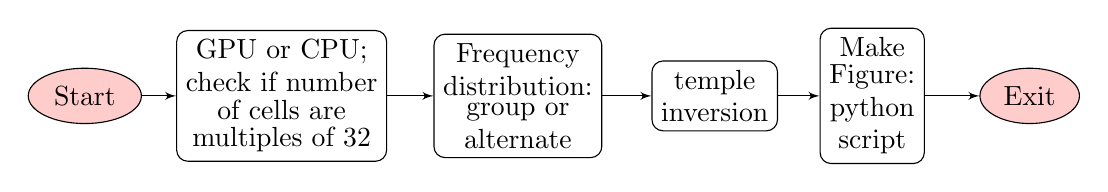
\begin{tikzpicture}[node distance = 3.0cm, auto]
%\begin{tikzpicture}
    \node [cloud] (start) {\shortstack{Start}};
    \node [rectangle, draw,
    text centered, rounded corners, right of=start, node distance =
2.5cm] (processors) {\shortstack{GPU or CPU; \\ check if number \\ of
cells are \\ multiples of 32}};
    \node [rectangle, draw,
   text centered, rounded corners, right of=processors, node distance
= 3.0cm] (freqdist) {\shortstack{Frequency\\ distribution:\\ group
or\\ alternate}};
   \node [rectangle, draw,
   text centered, rounded corners, right of=freqdist,node distance =
2.5cm] (tempinv) {\shortstack{temple\\ inversion}};
   \node [rectangle, draw,
   text centered, rounded corners, right of=tempinv, node distance =
2.0cm] (python) {\shortstack{Make\\ Figure: \\ python\\ script}};
   \node [cloud, right of=python, node distance = 2.0cm] (exit)
{\shortstack{Exit}};

    \path [line] (start) -- (processors);
    \path [line] (processors) -- (freqdist);
    \path [line] (freqdist) -- (tempinv);
    \path [line] (tempinv) -- (python);
    \path [line] (python) -- (exit);
\end{tikzpicture}
\caption{High Level activity diagram for main.cpp}
  \label{fig:fig3}
  \end{figure}
  
\subsection{Input parameters}

The inputs for the program are as follows.

\subsection{Subroutines}
\subsubsection{main.cpp}

A high level representation of the \texttt{main.cpp} can be viewed in
the \texttt{FWI.vpp} as a UML diagram.
\newline

The \texttt{main.cpp} initialises the MPI functions responsible for parallel
computations. Frequency distribution group and alternate are
determined here and depending on the user input, the objects are
created. Further, the main function creates the objects for the temple
inversion and calls the appropriate functions as seen in FWI\_temple.

\subsubsection{temple\_inversion}

The main part of the code can be seen in the
\texttt{temple\_inversion}. Over here, the Green's functions and
created and the mathematical model detailed in section 2 is executed.
A brief explanation of the functions can be seen as follows:

\paragraph{createGreens()}

This function creates an array of Green's functions of the Helmholtz
equations. It is called from the Inversion class and refers to the
equation \ref{eq:GreensFunc2d}.

\paragraph{CreateP0()}
$p_0$ is the field calculated with the known contrast and follows the
explanation given in section \ref{nonlinfupdate}.

\paragraph{createTotalField()}

After the initial approximation, first iterative $p_{tot}$ is
calculated here. This is done by calling the function calcfield(). In
this function, the equations defined in section \ref{nonlinfupdate} are calculated.
At first the incremental contrast sources are defined according to
equation \ref{eq:incrementalContrastSrcs} and then the $\phi_n$ is constructed. Based on
this \ref{eq:weightingFactorsField} is constructed. This step concludes the forward
modelling step.\\

Based on the input parameters, $\alpha$ is used
if $\alpha$ is 1 and is not used if it is set
to 0.

\paragraph{eq:calculateData()}
Once the total field $p_{tot}$ is obtained, the $p_{data}$ is
calculated according to \ref{eq:calculateData}.

\paragraph{Reconstruct()}
The reconstruct function might be the most important function of the
code. The code runs in an iterative loop to minimise the residuals.
According to tolerance values determined by the user and the max
number of iterations, the residuals are minimised in order to obtain
$p_{data}$. Once the residuals are minimised below the tolerance
level, the final model is obtained.\\

The Conjugate Gradient scheme detailed in section \ref{conjgrad} is coded here.

\paragraph{MakeFigure()}

Finally, the \texttt{MakeFigure()} function is called which calls a
python script to generate the figures.

\subsection{Parallelization: from a single CPU to Multiple and GPU}
The message passing interface (MPI) is a standardized means of
exchanging messages between multiple computers running a parallel
program across distributed memory.

In parallel computing, multiple computers - or even multiple processor
cores within the same computer - are called nodes.  Each node in the
parallel arrangement typically works on a portion of the overall
computing problem. The challenge then is to synchronize the actions of
each parallel node, exchange data between nodes and provide command
and control over the entire parallel cluster. The message passing
interface defines a standard suite of functions for these tasks.

For the FWI, the user sets in the input parameters, if GPU or CPU
should be used. This is already checked in the beginning of the code
and the appropriate functions corresponding to each are used. Further,
the user also sets whether the frequency distribution should be group
or alternate. This means that instead of splitting calculations over
frequency chunks, split them alternatively over frequency for a better
load balancing.

\section{\textcolor{orange}{Downloading, Installing and Running the Code}}

\subsection{Pre-requisites}
The prerequisite development tools needed can be installed using the following commands.

\begin{enumerate}
    \item \texttt{sudo apt-get install git}  
    \item \texttt{sudo apt-get install qt5-default}
    \item \texttt{sudo apt-get install libeigen3-dev}
    \item \texttt{sudo apt-get install python2.7-dev}
    \item \texttt{sudo apt-get install python2.7}
    \item \texttt{sudo apt-get install python-tk}
    \item \texttt{sudo apt-get install python-numpy}
    \item \texttt{sudo apt-get install python-matplotlib}

\end{enumerate}

\subsection{Cloning the Repository}
\noindent To clone the FWI repository using git,
\newline
\texttt{git clone -o redmine https://git.alten.nl/parallelized-fwi.git}
\newline
This will create a copy of the repository, in a folder named \textbf{parallelized-fwi}
\newline
Any branch as needed can then be checked out from inside the \texttt{parallelized-fwi} folder, e.g. the develop branch
\newline
\texttt{git checkout develop}

\subsection{Build/Run}
To build the project, first create a folder titled \textbf{build} outside the \textbf{parallelized-fwi} folder.
\newline
\texttt{NOTE: This folder should be exactly 1 level outside the parallelized-fwi folder.}
\newline
\texttt{mkdir Build}
\newline
\texttt{cd Build}
\newline
\texttt{cmake -DCMAKE\_BUILD\_TYPE=Release ../parallelized-fwi/}
\newline
\texttt{make -j4} (the flag -j is used to build in parallel)
\newline
Now, the individual scripts for the preProcessing and the processing part can be run as shown below:
\newline
\texttt{cd applications}
\newline
\texttt{cd preProcessing}
\newline
\texttt{./FWIPreProcess}
\newline
\texttt{cd ../processing}
\newline
\texttt{./FWIProcess}
\newline
The input parameters for the code are provided in the input card i.e. default.in. User can create his/her own input card with a new name e.g. \texttt{newCard.in}. To use this input card use the card name as an argument when running the executables, \texttt{./FWIPreProcess newCard} and \texttt{./FWIProcess newCard}.\newline

\noindent For post-processing (i.e. generation of image using the estimated chi values), the python script \texttt{imageCreator\_CMake.py} can be used. This script is located inside the \textbf{parallelized-fwi} folder and can used as,
\newline
\texttt{python imageCreator\_CMake.py}
\newline
The pre-processing, processing and the image creation step can all be grouped together using the python wrapper \texttt{wrap\_FWI\_CMake.py} located inside the \textbf{parallelized-fwi} folder.
\newline
\texttt{python wrap\_FWI\_CMake.py}

\section{Results and Analysis - example: Temple Reservoir}

The example chosen for the FWI code is the logo of the Delphi
research consortium. The logo includes a
Greek temple consisting of four major
pillars under a triangularly shaped roof, as shown in Figure \ref{fig:fig4}.
Additionally we added a layer below the temple to represent the
basement. The whole structure is embedded in a homogeneous background
which carries waves at a
uniform acoustic velocity of
$c_0 = 2000 m/s$.
The temple material's carriage speed is $c = 2218 m/s$.
In the original data in \texttt{temple.txt}, you can see a list of
zeros and \texttt{1.869...e-01}. The zeros are the background's
contrast ``with itself'' and the 1.869...e-01 the result of $1-
{(\frac{2000}{2218})}^2$.
The Results obtained from running the FWI code can be seen in the
following figures:
\begin{figure}
\centering
 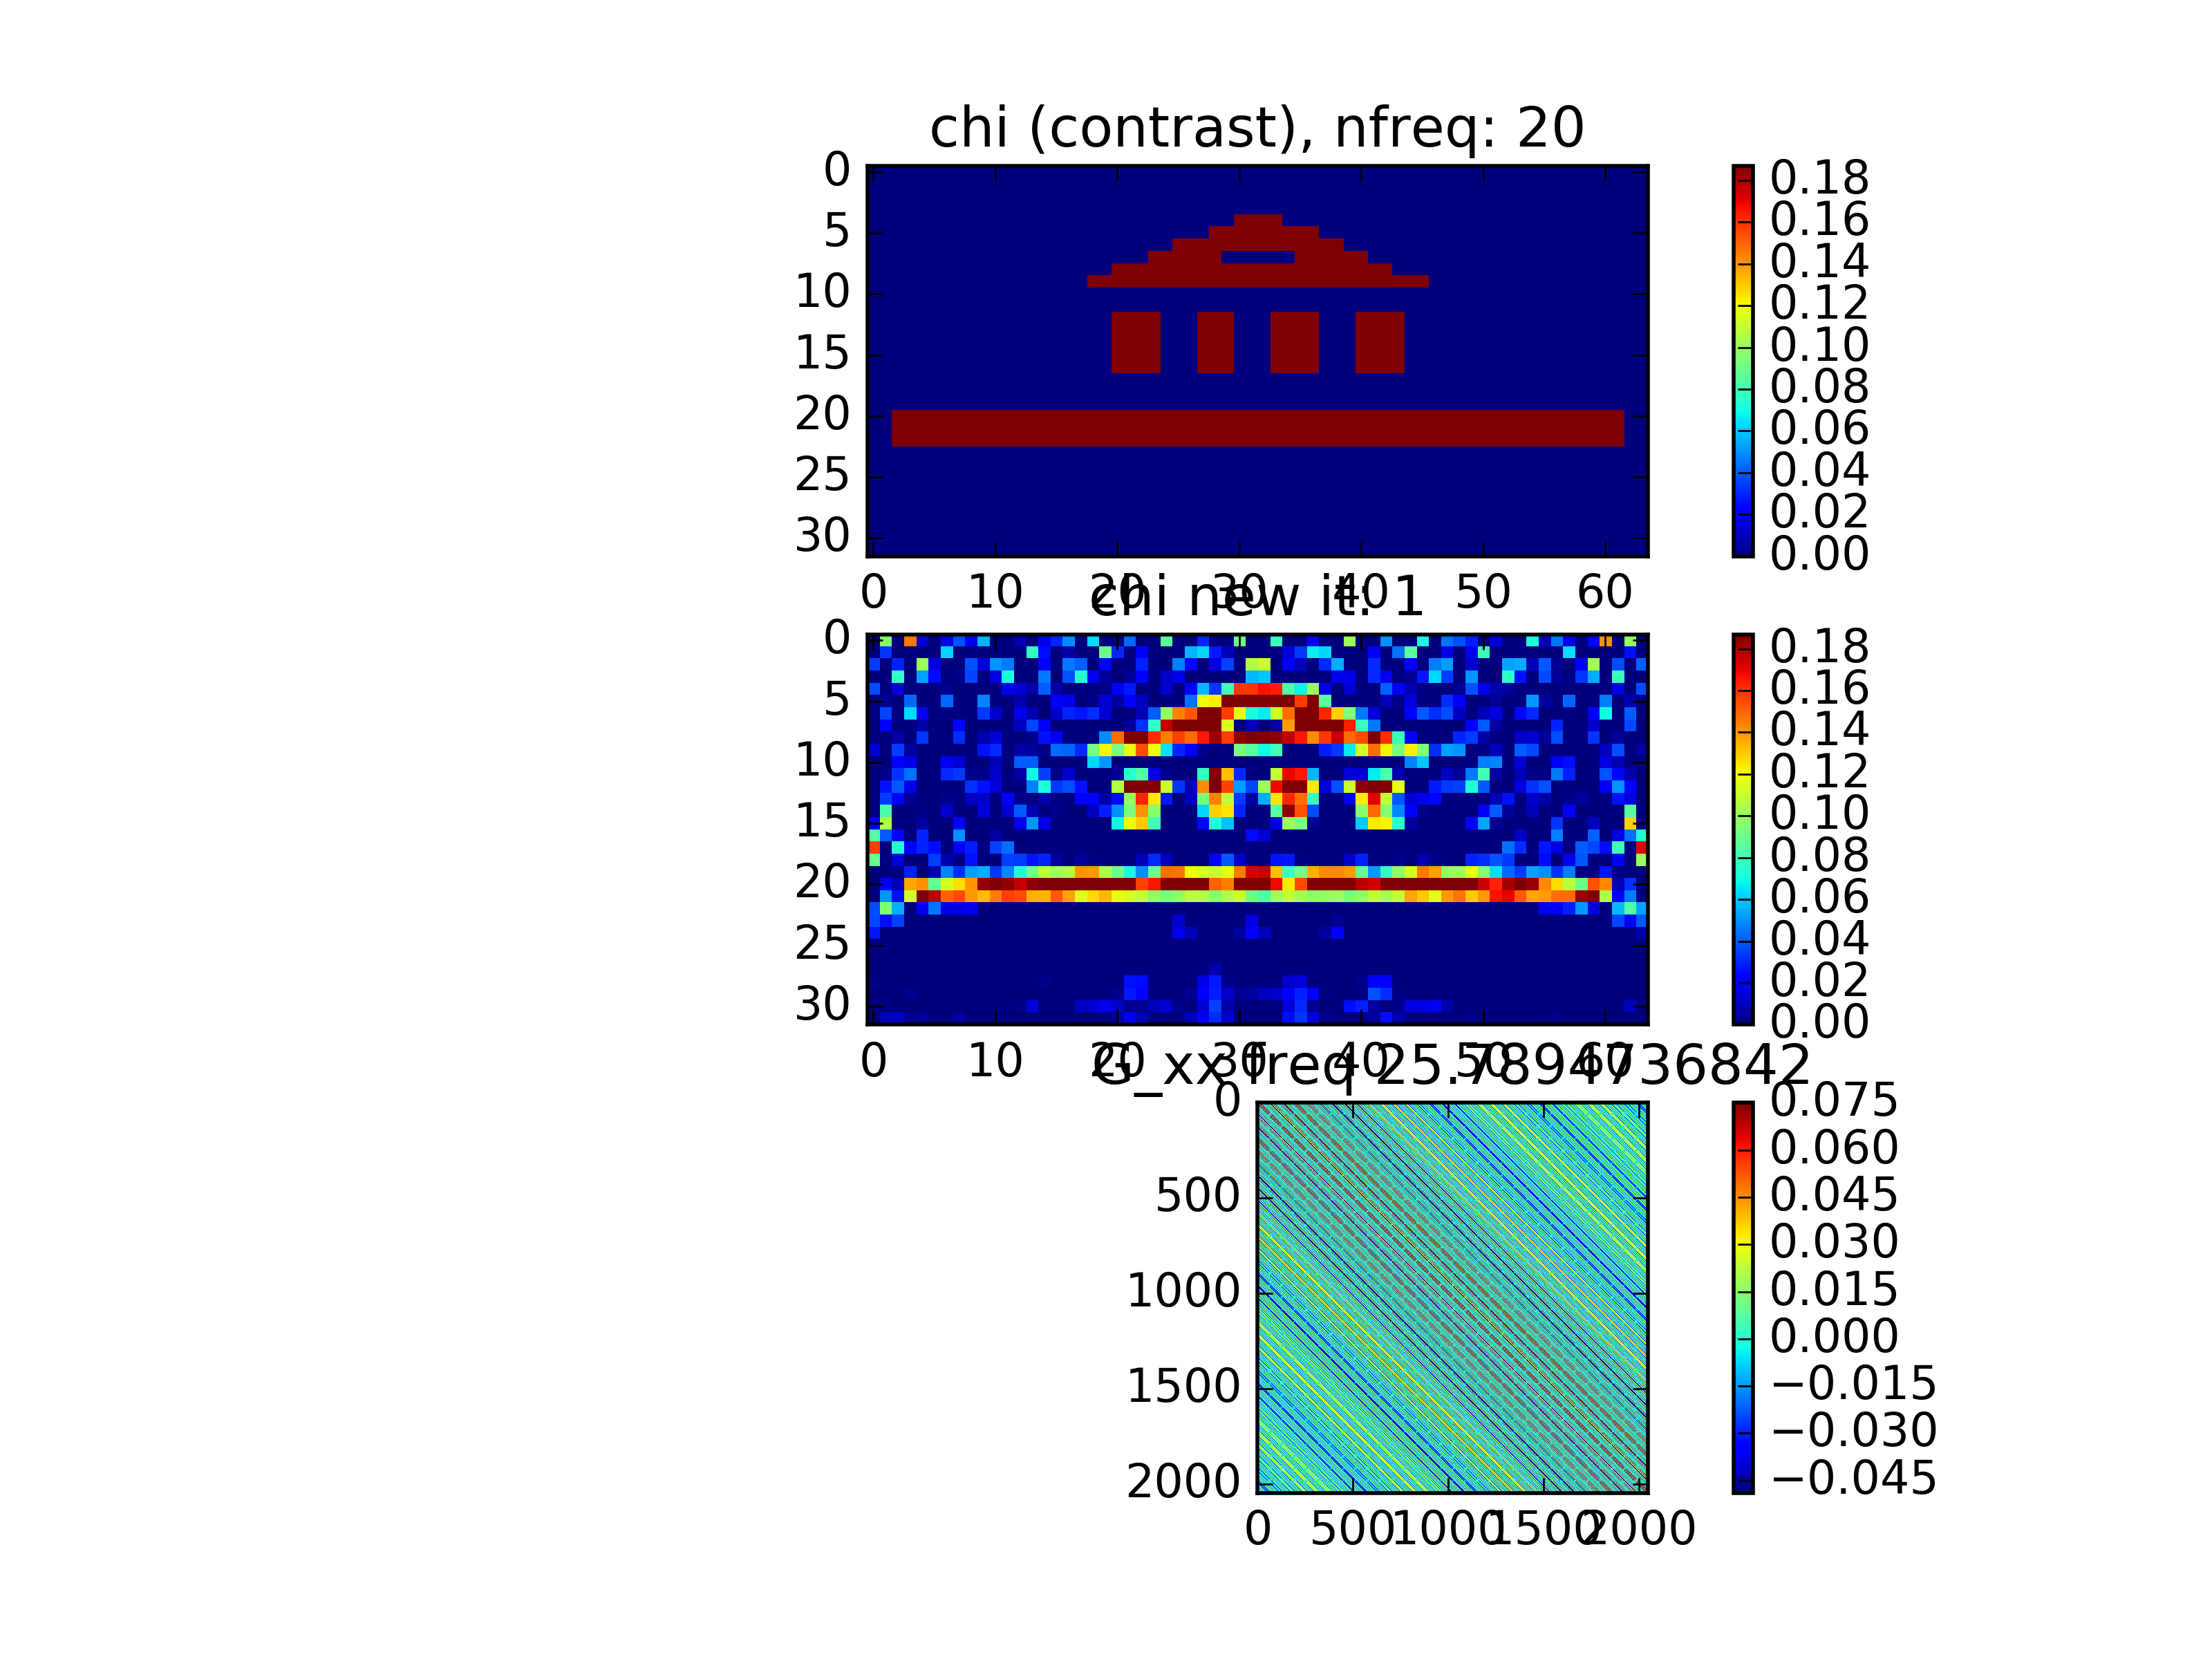
\includegraphics[scale=0.75]{Chi_est_it00.png}
  \caption{Chi estimation Result 1}
  \label{fig:fig4}
 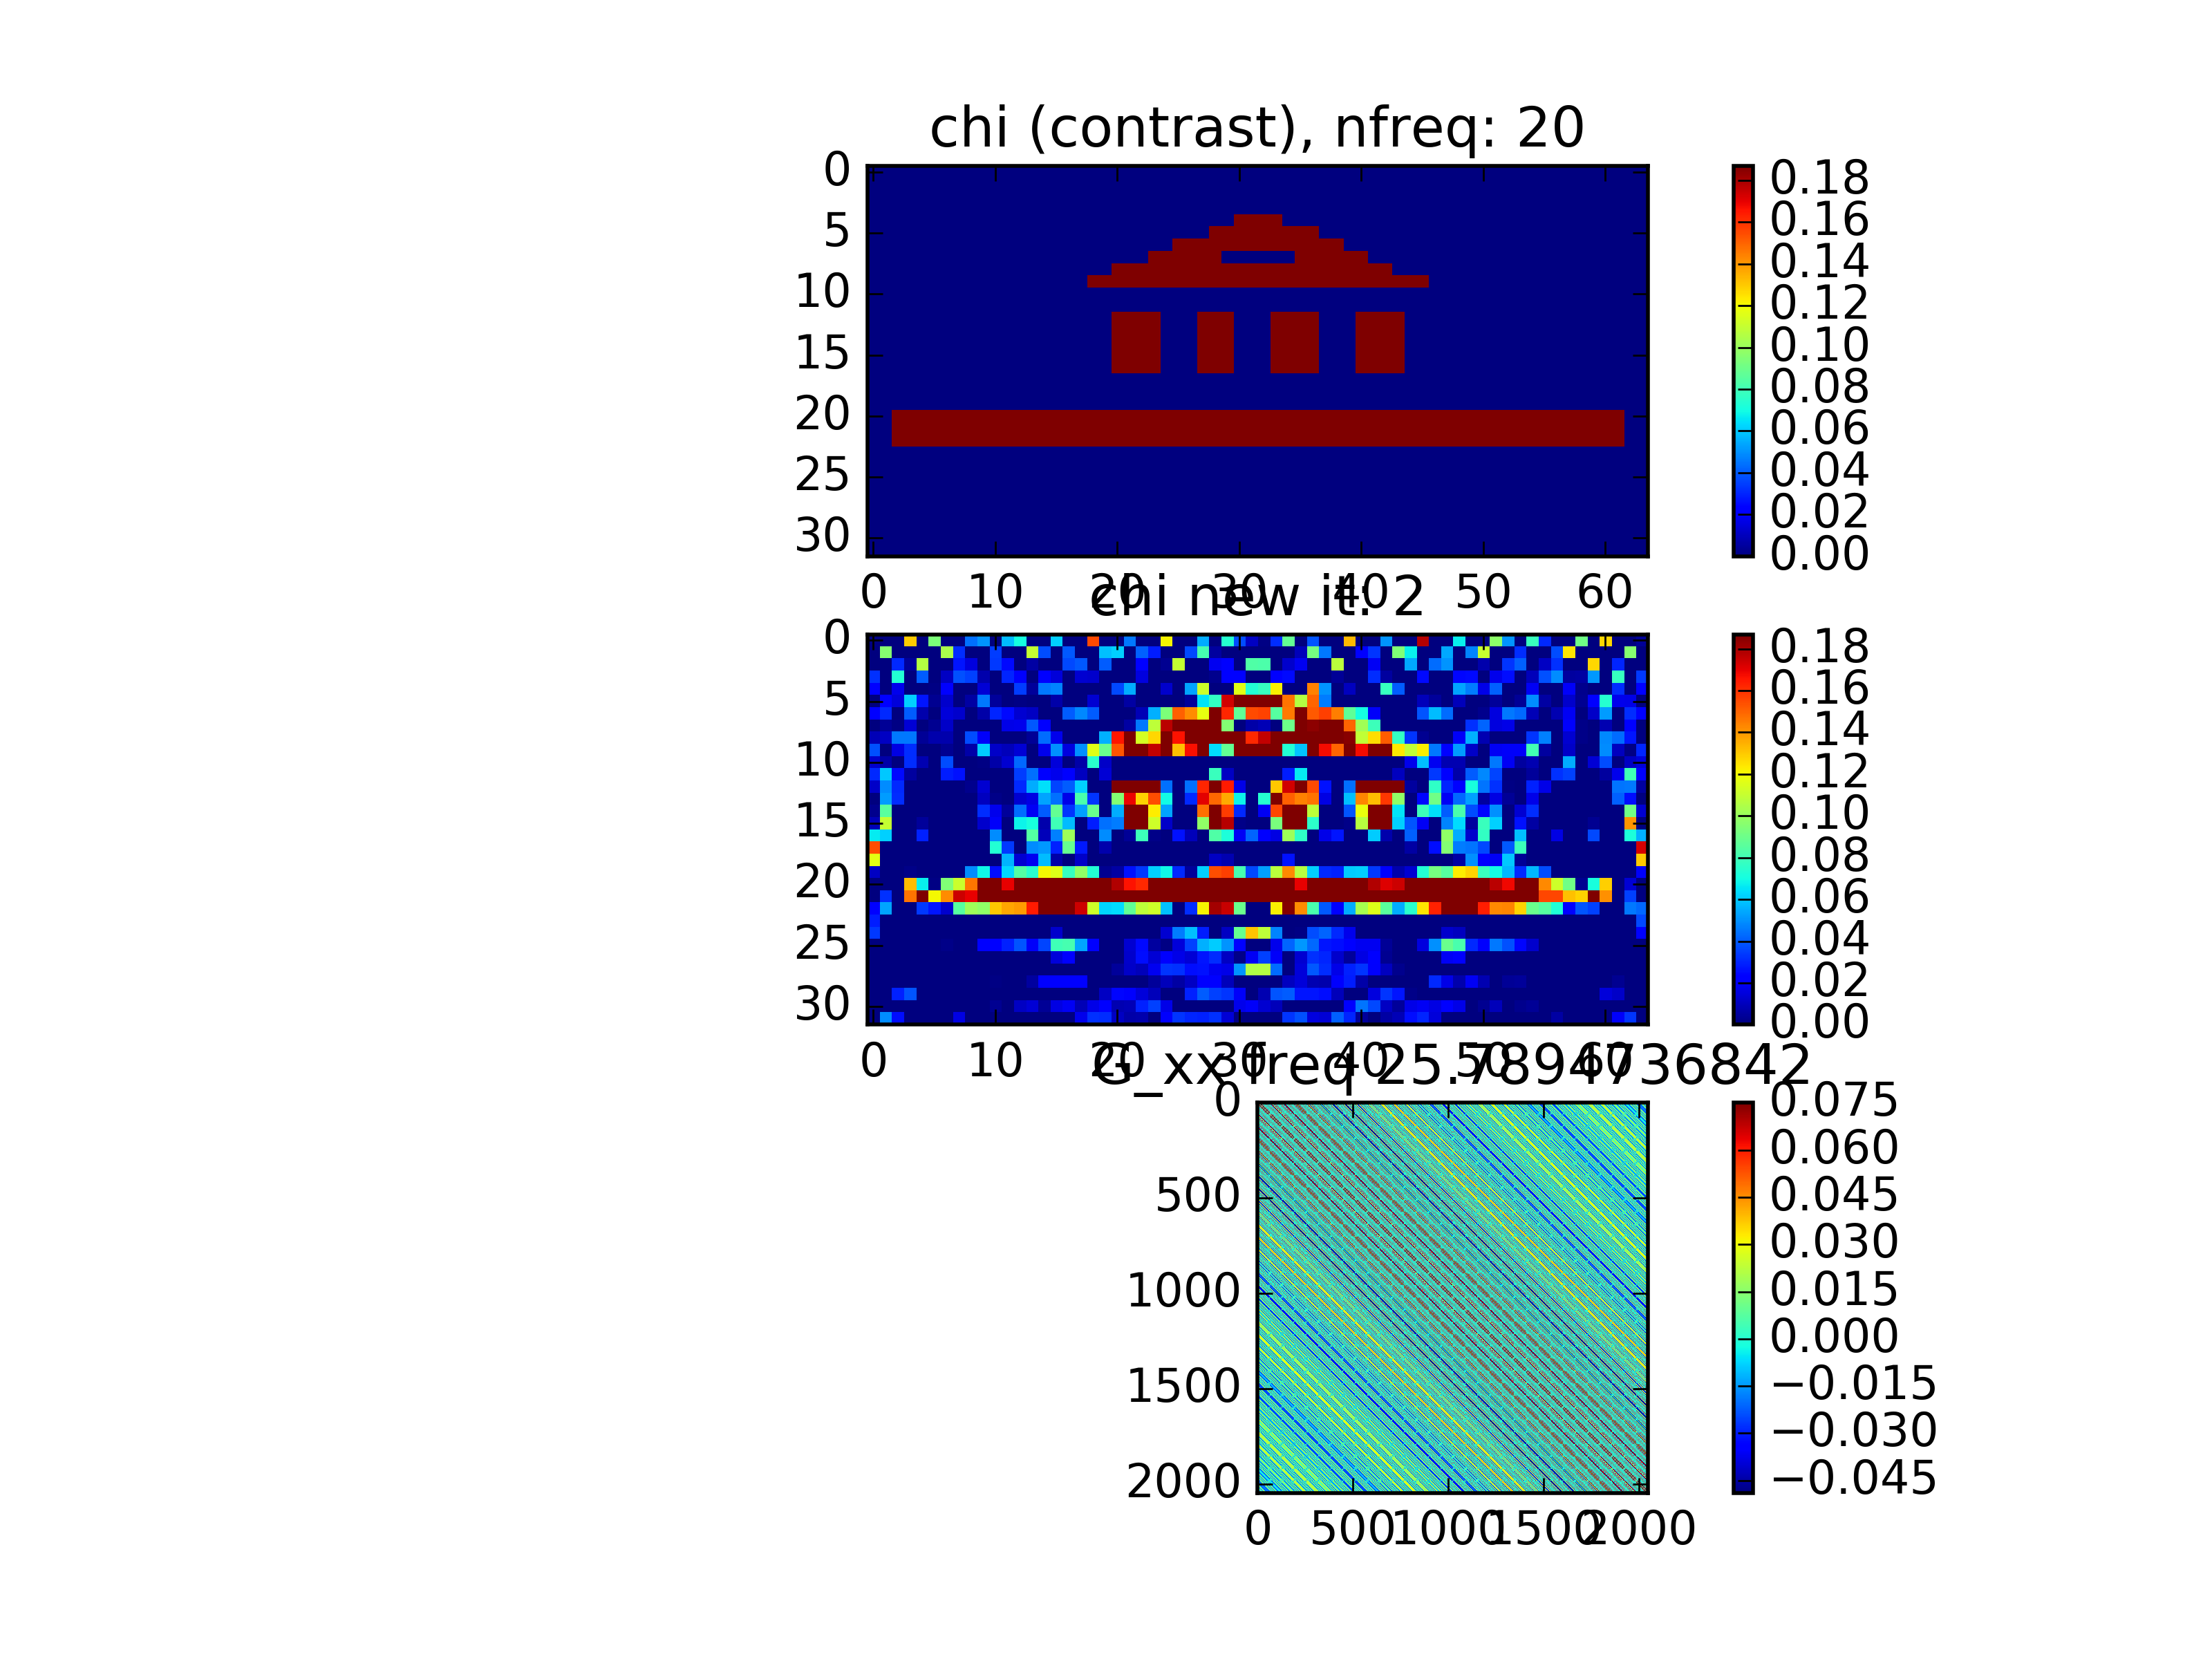
\includegraphics[scale=0.75]{Chi_est_it01.png}
  \caption{Chi estimation Result 2}
  \label{fig:fig5}
\end{figure}

\begin{figure}
\centering
 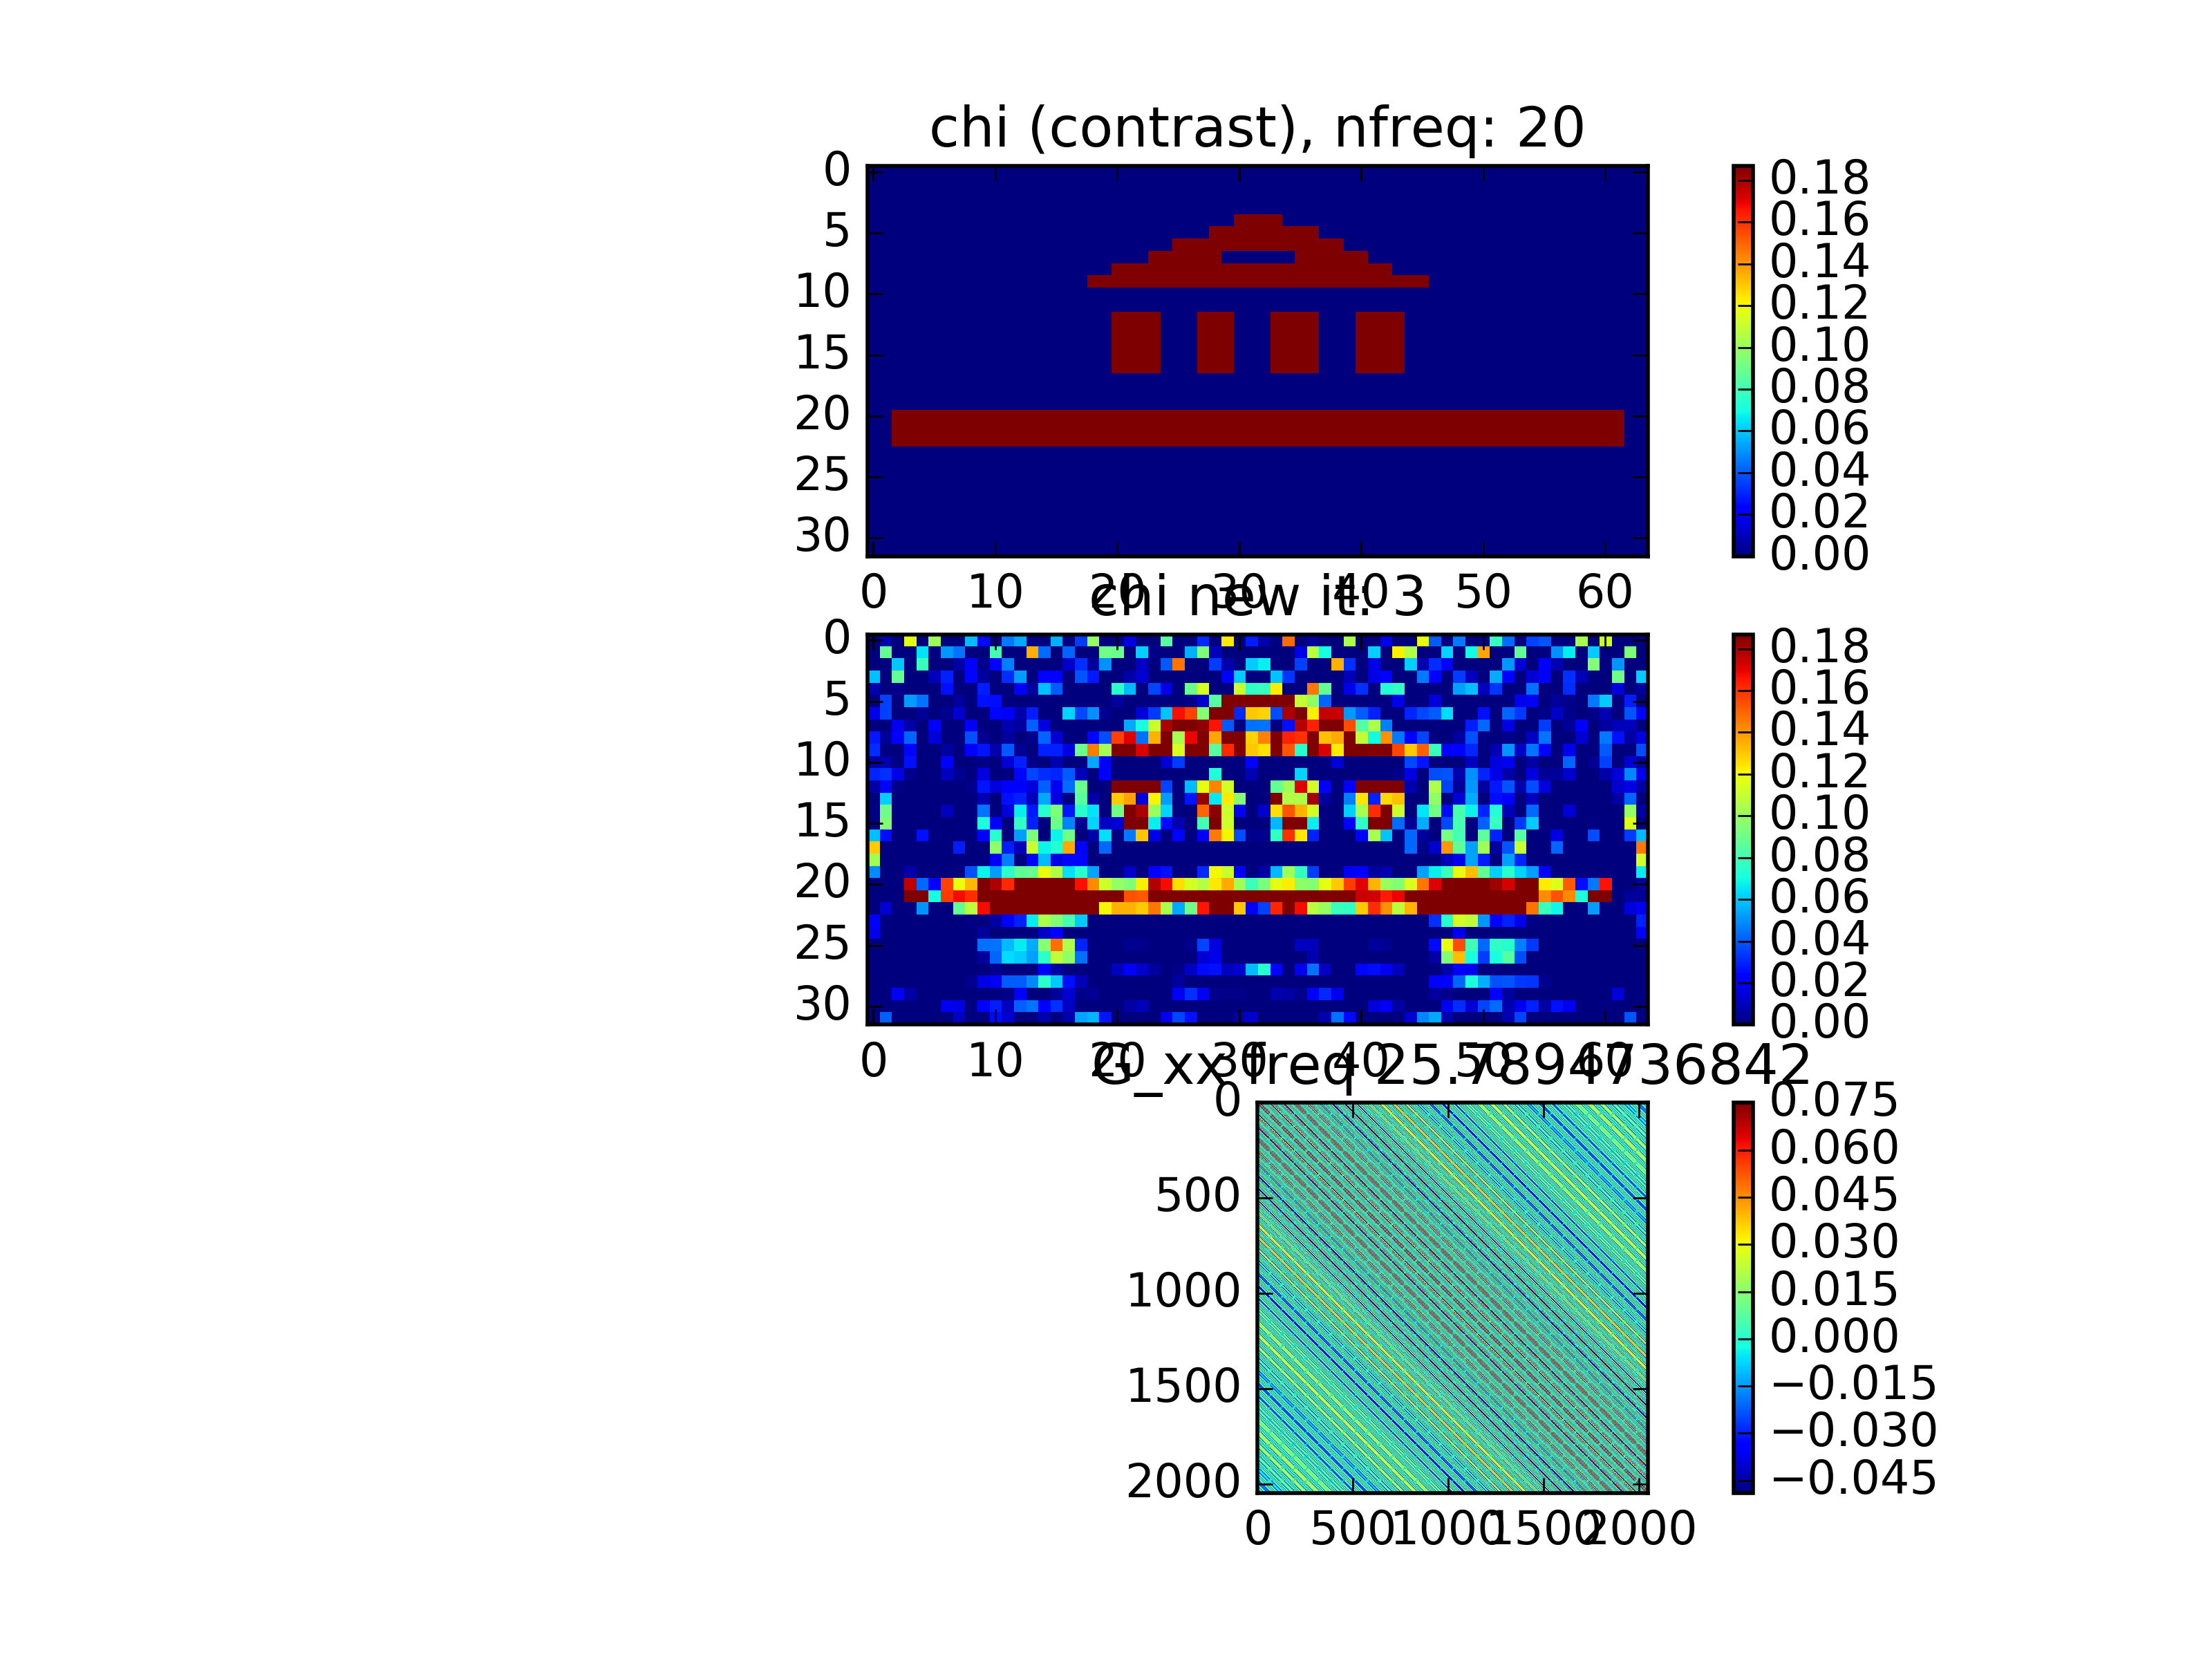
\includegraphics[scale=0.75]{Chi_est_it02.png}
  \caption{Chi estimation Result 3}
  \label{fig:fig6}
 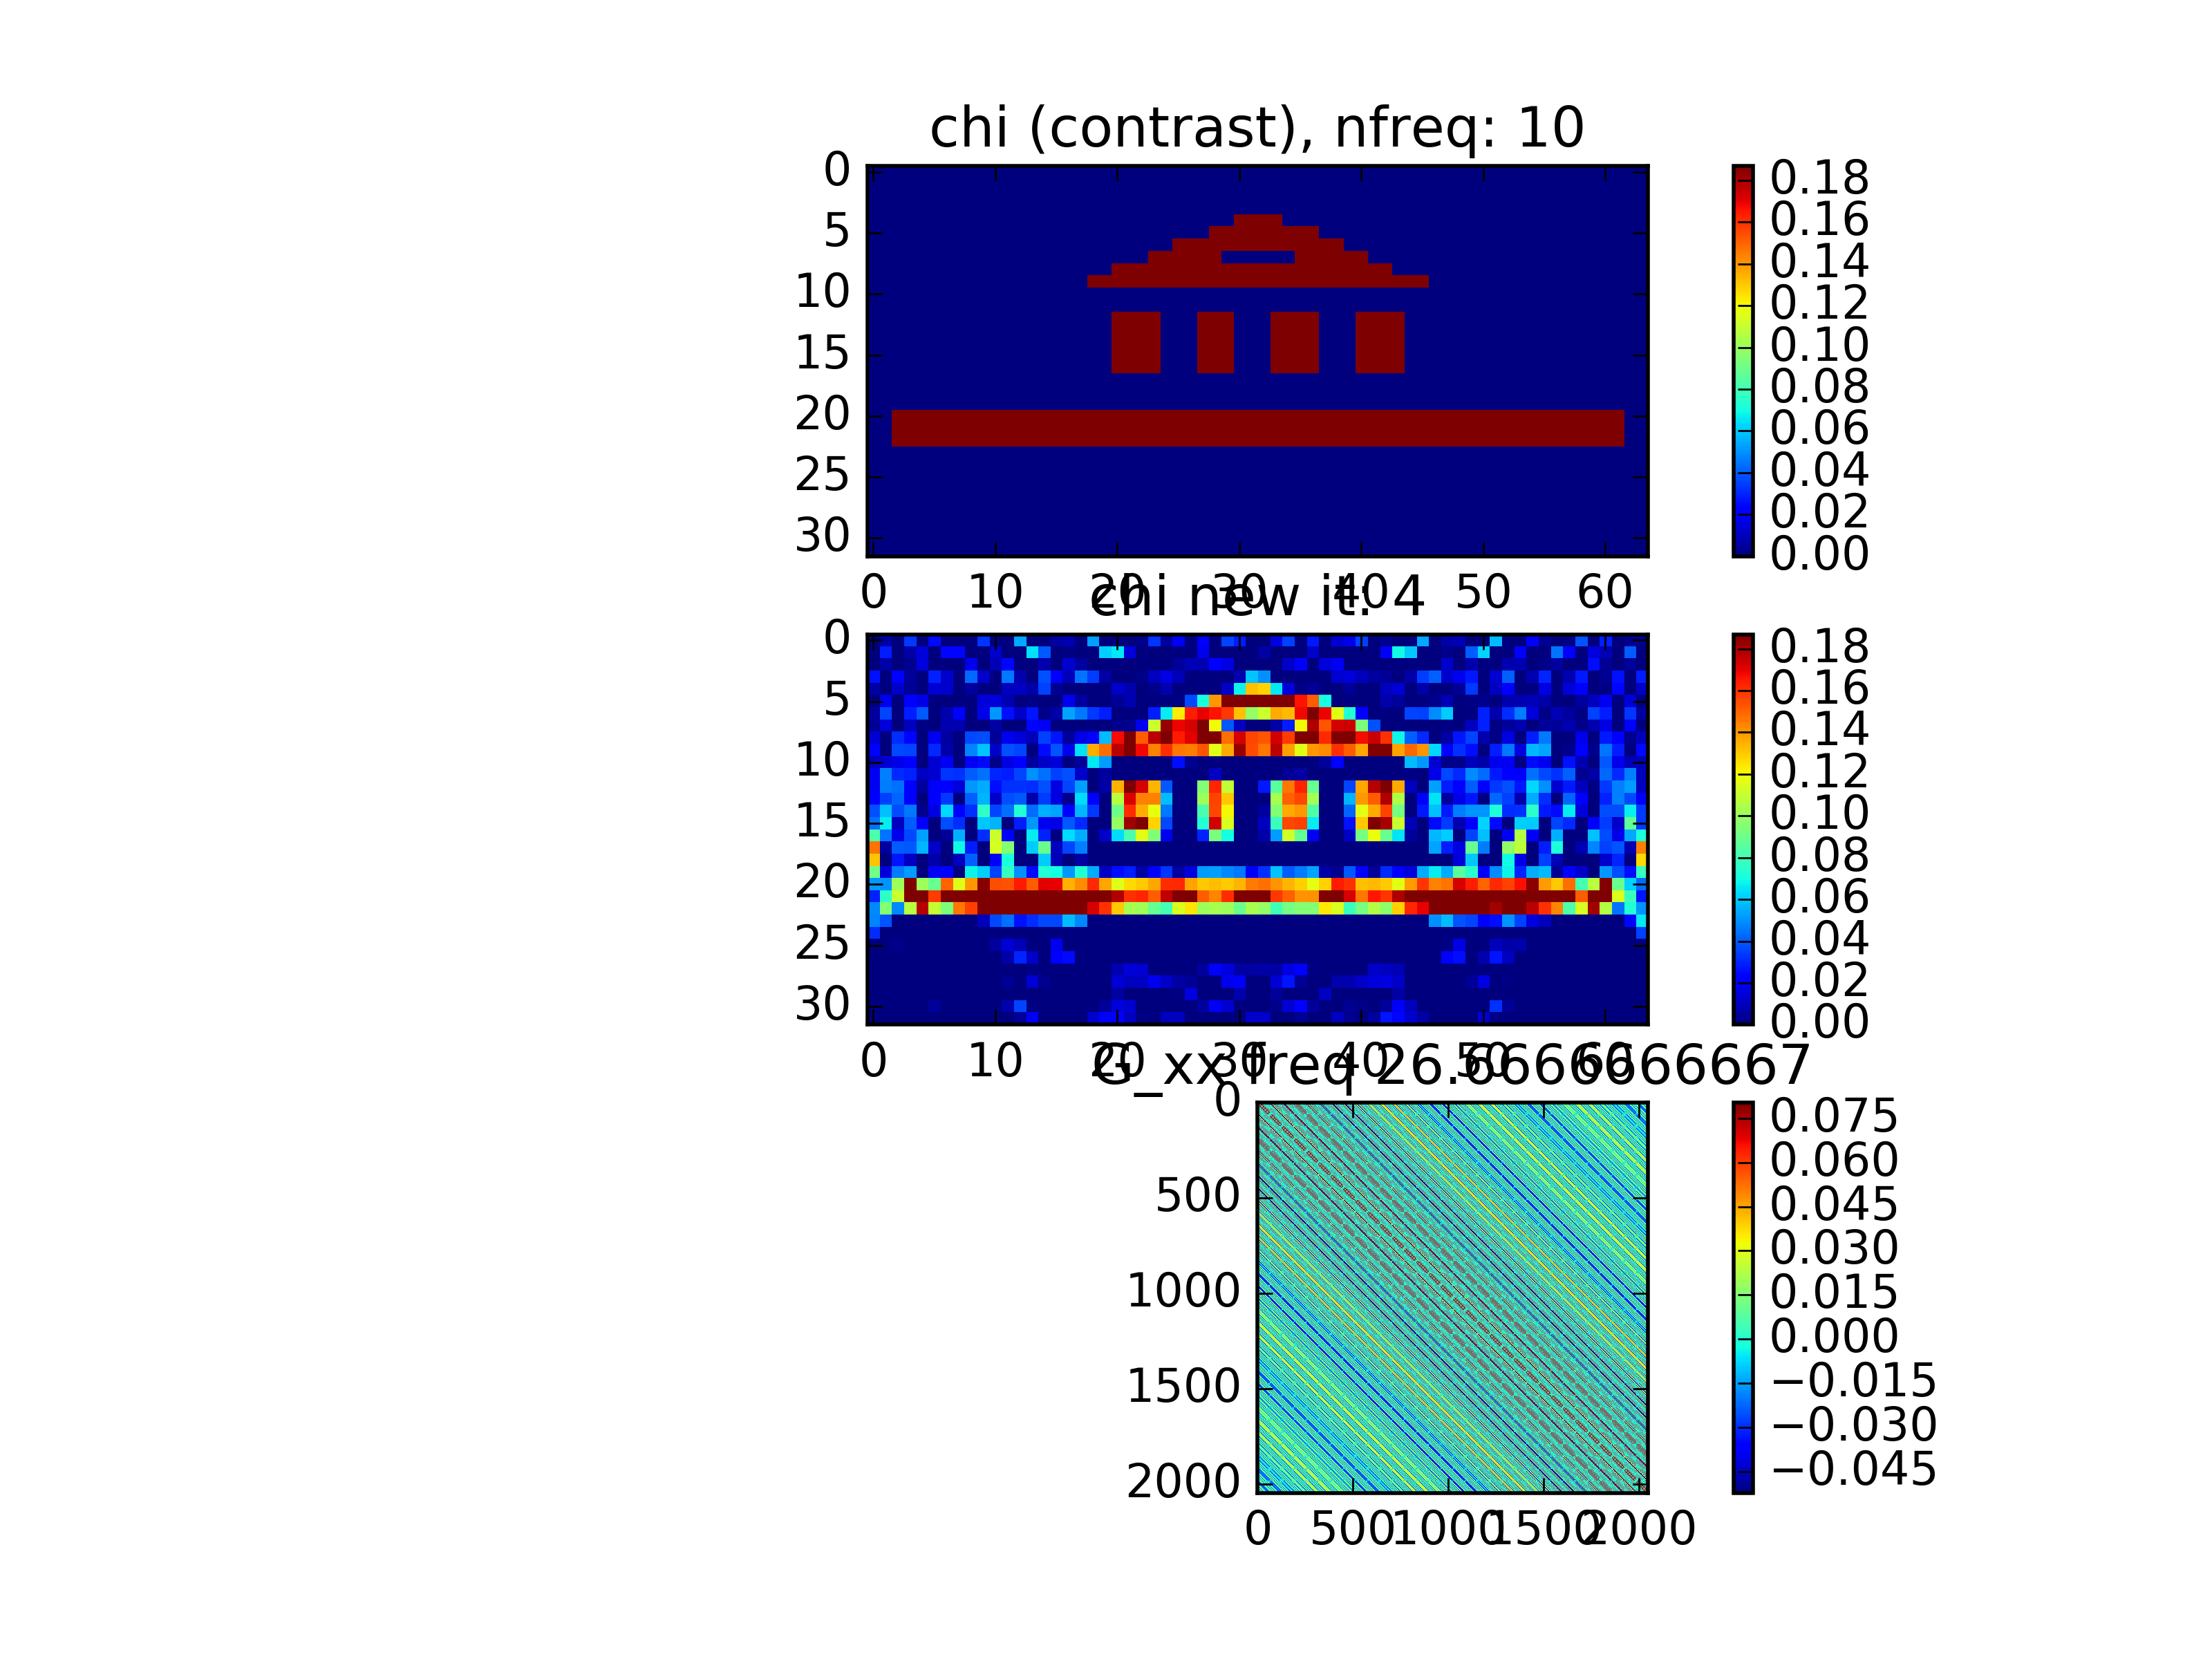
\includegraphics[scale=0.75]{Chi_est_it03.png}
  \caption{Chi estimation Result 4}
  \label{fig:fig7}
\end{figure}

\begin{figure}
\centering
 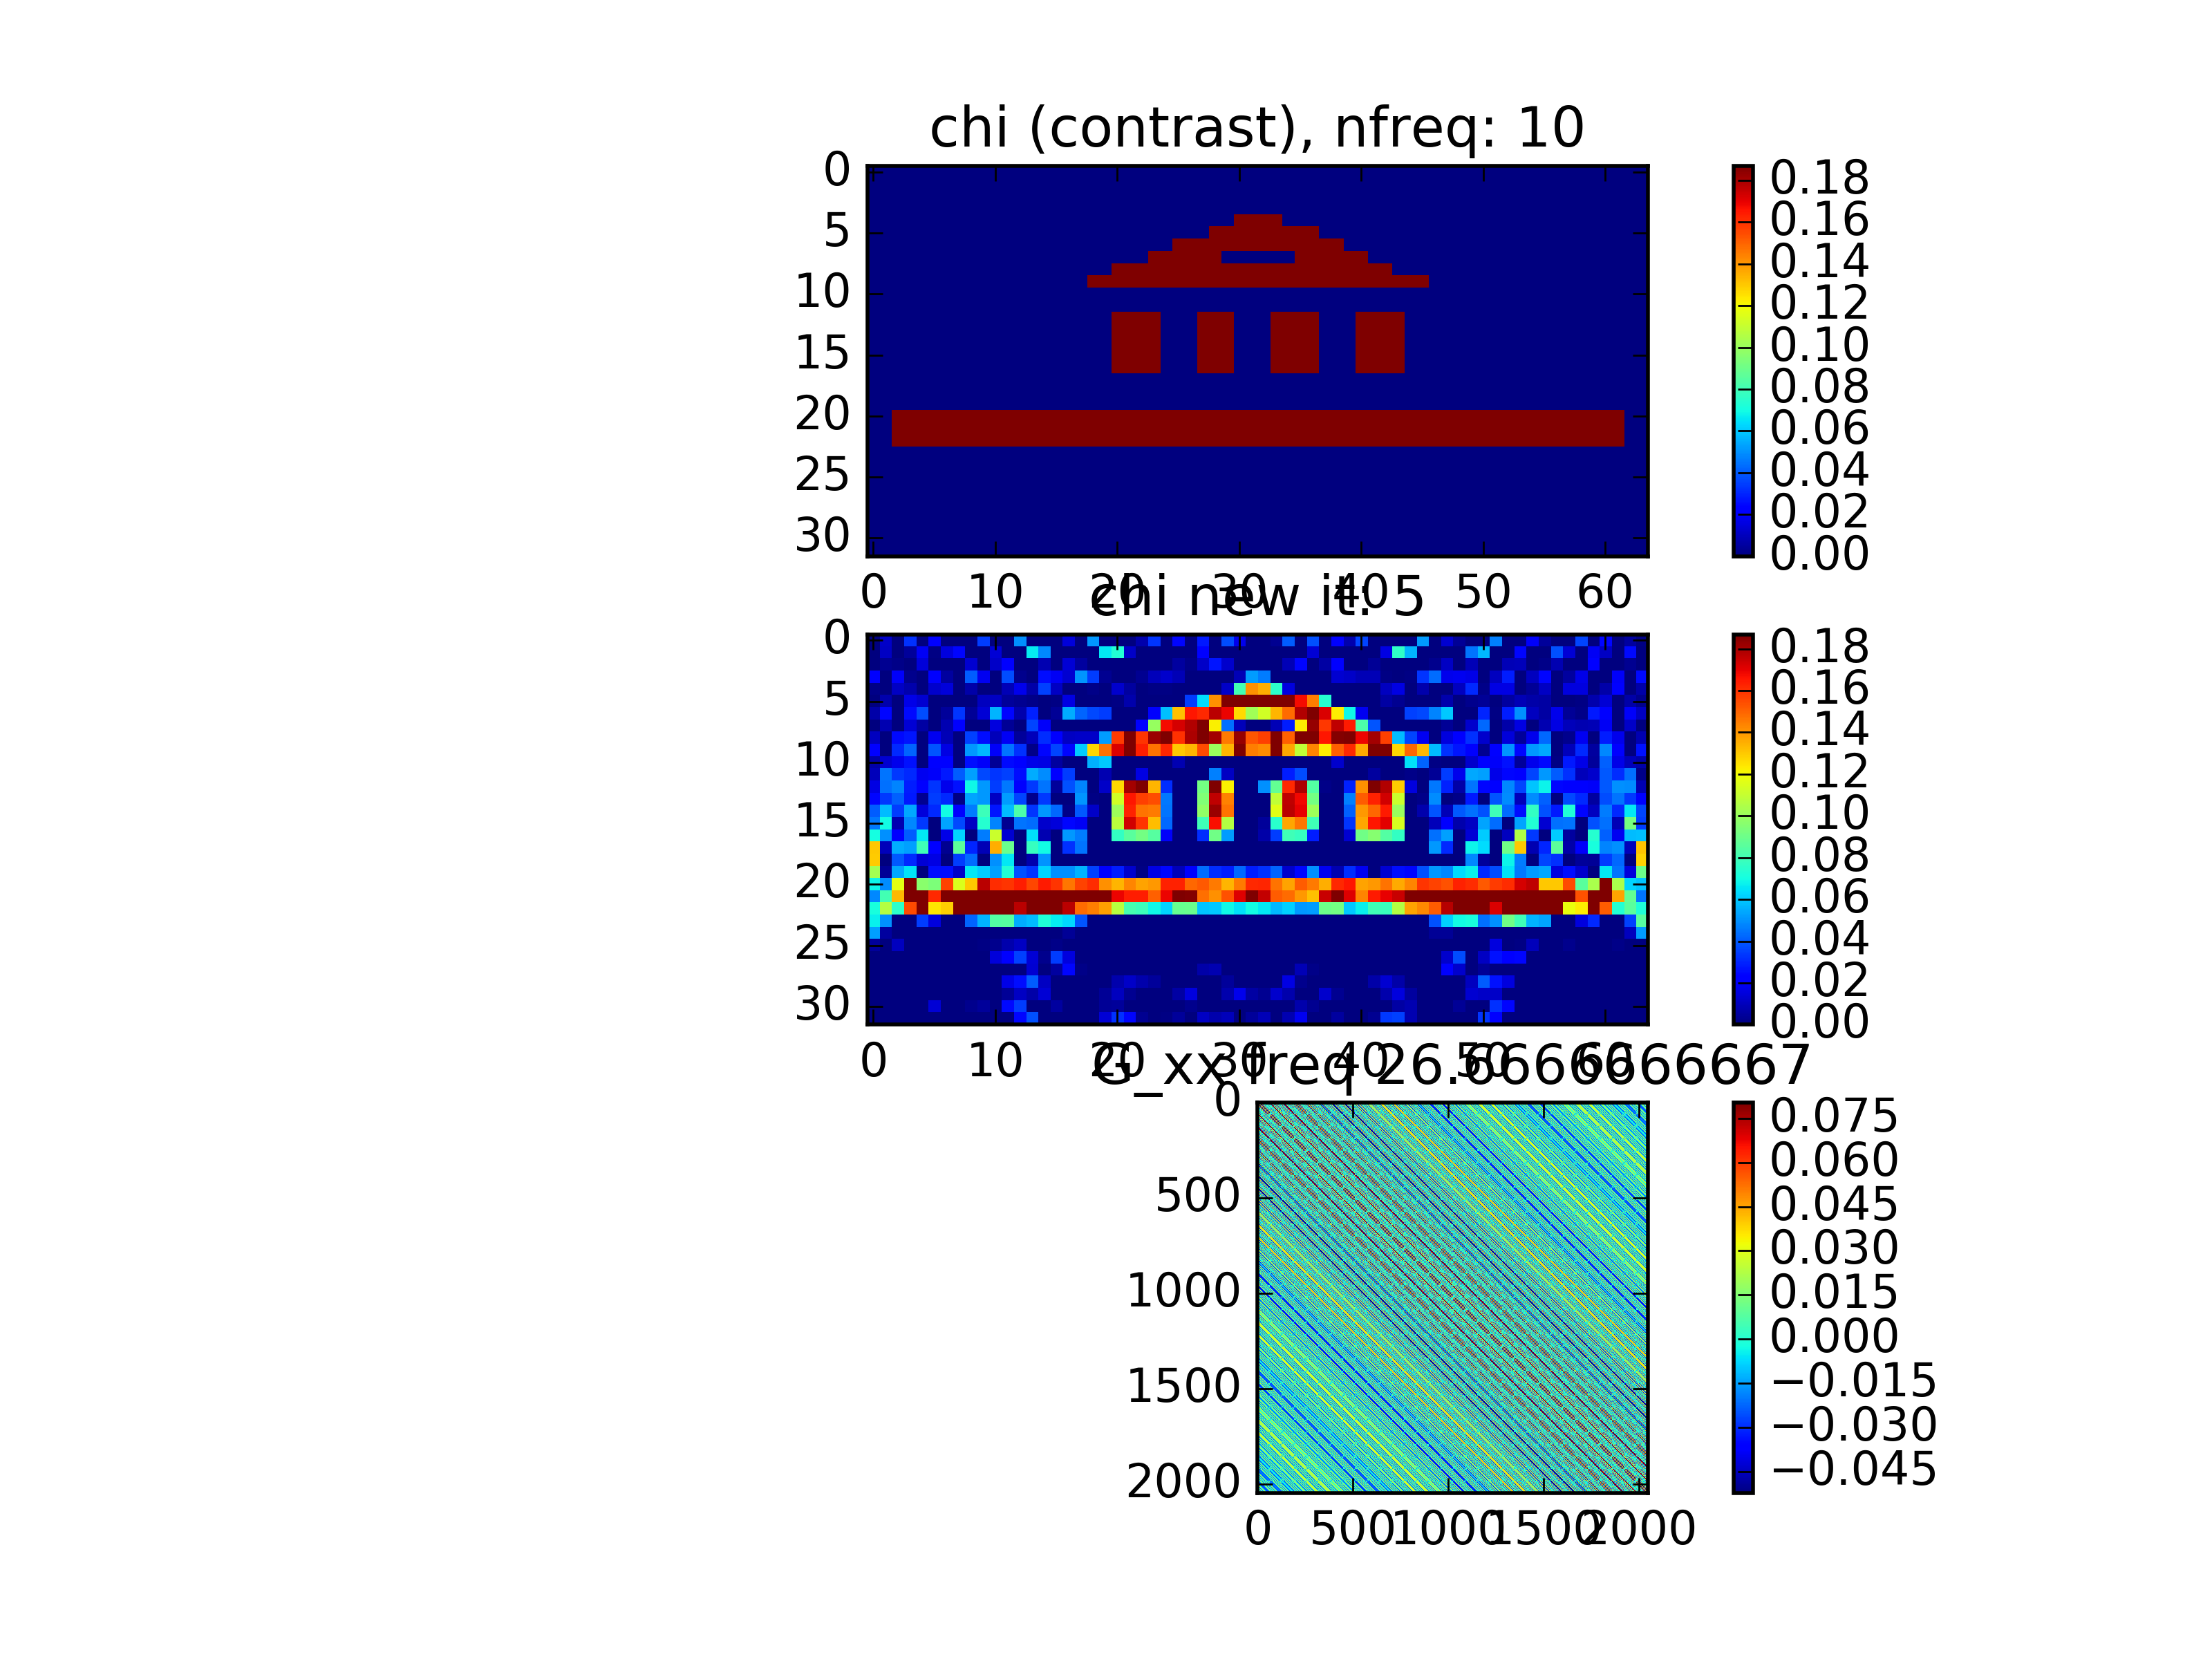
\includegraphics[scale=0.75]{Chi_est_it04.png}
  \caption{Chi estimation Result 5}
  \label{fig:fig8}
\end{figure}

\newpage
\nocite{*}
\bibliographystyle{abbrv}
\bibliography{bibliography}

\clearpage

\appendix
\section{Appendices}
\subsection{Derivation of the functional derivative of the error functional}
\label{deriveerrorfunctional}
\begin{eqnarray*}
\partder{F(\mathbf{\chi}, \mathbf{d})}{\mathbf{\chi}} & = &
\lim_{\epsilon \rightarrow 0} \frac{F(\mathbf{\chi} + \epsilon
\mathbf{d}) - F(\mathbf{\chi})}{\epsilon} \\
& = & \lim_{\epsilon \rightarrow 0} \frac{\eta}{\epsilon} \int
\left(p_{\text{data}} - \left[\mathcal{K}_\chi \right] - \epsilon
\left[\mathcal{K}_\mathbf{d} \right] \right) \left(p_{\text{data}} -
\left[\mathcal{K}_\chi \right] - \epsilon \left[\mathcal{K}_\mathbf{d}
\right] \right)^{\dagger}\\
& \, \, \, \, \, \, \, \, \, \, \, \, \, \, \, \, \, \, \, \, \, \, \,
\, \, \, \, - & \left(p_{\text{data}} - \left[\mathcal{K}_\chi \right]
\right) \left(p_{\text{data}} - \left[\mathcal{K}_\chi \right]
\right)^{\dagger} \df{\xs} \df{\xr} \df{\omega} \\
& = & -\lim_{\epsilon \rightarrow 0} \frac{\eta}{\epsilon} \int
\epsilon \left[ \left[\mathcal{K}_\mathbf{d} \right]
\left(p_{\text{data}} - \left[\mathcal{K}_\chi \right]
\right)^{\dagger} + \left[\mathcal{K}_\mathbf{d} \right]^{\dagger}
\left(p_{\text{data}} - \left[\mathcal{K}_\chi \right] \right) \right]
\\
& \, \, \, \, \, \, \, \, \, \, \, \, \, \, \, \, \, \, \, \, \, \, \,
\, \, \, \, - & \epsilon^2 \left[\mathcal{K}_\mathbf{d} \right]
\left[\mathcal{K}_\mathbf{d} \right]^{\dagger} \df{\xs} \df{\xr}
\df{\omega} \\
& = & -2 \eta \int \real{\left[\mathcal{K}_\mathbf{d} \right]
\left(p_{\text{data}} - \left[\mathcal{K}_\chi \right]
\right)^{\dagger}} \df{\xs} \df{\xr} \df{\omega} \\
& = & -2 \eta \int \real{\left[\mathcal{K}_\mathbf{d} \right](\xr,
\xs, \omega)^{\dagger} r (\xr, \xs, \omega)} \df{\xs} \df{\xr}
\df{\omega}
\end{eqnarray*}

\subsection{Prefactors of the Total Cost Equation}
\label{totalcostprefactors}
\begin{align} \label{eq:totalCostA2} \mathcal{A}_2 = \eta \int \int \int
\mid \mathcal{K} \zeta_n \mid^2 d\vec{x_s}d\vec{x_r}d\omega\\
\tag*{\texttt{totalCostA2}}
\end{align}

\begin{align} \label{eq:totalCostA1} \mathcal{A}_1 = -2 \eta \real{\int
\int \int r^{\star}_{n-1} \mid \mathcal{K} \zeta_n \mid
d\vec{x_s}d\vec{x_r}d\omega} , \hat{E}\\
\tag*{\texttt{totalCostA1}}
\end{align}

\begin{align} \label{eq:totalCostA0} \mathcal{A}_0 = \eta \int \int \int
\mid r_{n-1} \mid^2 d\vec{x_s}d\vec{x_r}d\omega =
\mathcal{F}^{data}_{n-1} , \hat{E}\\
\tag*{\texttt{totalCostA0}}
 \end{align}

\begin{align} \label{eq:totalCostB2} \mathcal{B}_2 = \mid \mid b_n \nabla
\zeta_n \mid \mid^{2}_D , \hat{E}\\
\tag*{\texttt{totalCostB2}}
\end{align}

\begin{align} \label{eq:totalCostB1} \mathcal{B}_1 = 2 < b_n
\nabla\chi^{n-1}, b_n \nabla \zeta_n >_D, \hat{E}\\
\tag*{\texttt{totalCostB1}}
\end{align}

\begin{align} \label{eq:totalCostB0} \mathcal{B}_0 = \mid \mid b_n \nabla
\chi^{n-1} \mid \mid^{2}_D + \delta^{2}_{n-1} \mid \mid b_n \mid
\mid^{2}_D\\
\tag*{\texttt{totalCostB0}}
\end{align}

\section{Absorbing Boundary Conditions}\label{sec:ABC}
\subsection{First Order ABC}
As an alternative Absorbing Boundary Conditions (ABC) can be used to (partially) prevent reflections. First we assume that the index of refraction $n(\x)\equiv C_1$ close to the boundary for some $C_1\in \mathbb{R}$. The main idea of ABC is that close to the boundary the solution to the full problem can be approximated by a plane wave that propagates in a direction normal to the boundary \cite{LectNotes}, i.e.

\begin{equation}
u(\x) \approx Ce^{i\omega C_1 \hat{\n}\cdot \x},
\end{equation}

where $\hat{\n}$ denotes the outward pointing normal of the boundary. Now consider, for example, the upper boundary $\Gamma_0$. We want the ABC to block all outgoing waves, so that they cannot cause reflections. Since we assumed that waves close to the boundary can be approximated by a wave traveling in a direction normal to the boundary, we want the waves with direction $[0,-1]^\top$ to be blocked. Now

\begin{equation}
\frac{\partial u}{\partial \hat{\n}} -i\omega C_1 u = i\omega CC_1e^{-i\omega C_1z} - i\omega CC_1e^{-i \omega C_1 z} = 0
\end{equation}

for $\hat{\n}=[0,-1]^\top$ and for all $C\in\mathbb{R}$\footnote{Since, for $\hat{\n} = [\hat{n}_1,\hat{n}_2]^\top$, we have 
	\begin{equation*}
	\frac{\partial u}{\partial \hat{\n}} -i\omega nu= \nabla u\cdot \hat{\n} -i\omega nu= i\omega nC (\hat{n}_1^2 e^{i\omega n(\hat{n}_1x+\hat{n}_2z)} + \hat{n}_2^2e^{i\omega n(\hat{n}_1x+\hat{n}_2z)})-i\omega nCe^{i\omega n(\hat{n}_1x+\hat{n}_2z)}
	\end{equation*}}. Hence the ABC can be formulated as

\begin{equation}
\frac{\partial u}{\partial \hat{\n}} - i\omega nu=0,
\end{equation}

The ABC formulated above are first order accurate in the angle at which the wave strikes the boundary \cite{AbsorpationRates}.

\subsubsection{Discretization}
For points on the boundary not all neighbours exist. Consider, for example, the top left boundary point. There $u_{i-1,j}$ and $u_{i,j+1}$ do not exist. From the boundary conditions it follows that

\begin{eqnarray}
&& \frac{\partial u}{\partial \hat{\n}} - i\omega nu = -\frac{\partial u}{\partial x} - i\omega nu =0\\
&\leadsto& -\frac{u_{i+1,j}-u_{i-1,j}}{2h_x}-i\omega n_{ij} u_{ij}=0\\
&\implies& u_{i-1,j} = 2h_xi\omega n_{ij}u_{ij}+u_{i+1,j}
\end{eqnarray}

where $\hat{\n}=[-1,0]^\top$ is the outward pointing normal and 

\begin{eqnarray}
&& \frac{\partial u}{\partial \hat{\n}} - i\omega nu = -\frac{\partial u}{\partial z} - i\omega nu =0\\
&\leadsto& -\frac{u_{i,j+1}-u_{i,j-1}}{2h_z}-i\omega n_{ij} u_{ij}=0\\
&\implies& u_{i,j-1} = 2h_zi\omega n_{ij}u_{ij}+u_{i,j+1}
\end{eqnarray}

where $\hat{\n}=[0,-1]^\top$ is the outward pointing normal (since the positive $z$ direction is downwards). Here we used a central difference discretization. By substituting these relations into \cref{eqn:discret} the final discretization for the boundary point is obtained. 

\subsection{Second Order ABC}
To improve the absorption rate of the ABC, we will consider ABC which are second order accurate in the angle at which the wave strikes the boundary \cite{AbsorpationRates}. They can be formulated as follows.

\begin{equation} \label{eqn:SecondOrderABC}
\frac{\partial u}{\partial \hat{\n}} - in\omega u - \frac{i}{2\omega n}\frac{\partial^2 u}{\partial \s^2}=0,
\end{equation}

where $\s$ denotes the vector tangential to the boundary (positive or negative direction does not matter). In the corner specials ABC apply \cite{SecondOrderCorner}

\begin{equation}
\frac{\partial u}{\partial \hat{\s}}-\frac{3}{2}i\omega nu=0,
\end{equation}

where $\hat{\s}$ denotes the vector which is the sum of the tangential outward pointing vectors in the $x$ and $z$ directions.

\subsubsection{Discretization}
Similar to the first order discretization, at the boundary we need to find an expression for the ghost points. Consider, for example, the top boundary ($z=0$). Here $\hat{\n}=[0,-1]^\top$ and $\s=[\pm 1,0]$. Now \cref{eqn:SecondOrderABC} can be discretized as follows.

\begin{eqnarray}
&&\frac{\partial u}{\partial \hat{\n}} - in\omega u - \frac{i}{2\omega n}\frac{\partial^2 u}{\partial \s^2}= -\frac{\partial u}{\partial z} - in\omega u - \frac{i}{2\omega n}\frac{\partial^2 u}{\partial x^2}=0\\
&\leadsto& -\frac{u_{i,j+1}-u_{i,j-1}}{2h_z} - i\omega n_{ij}u_{ij}-\frac{i}{2\omega n_{ij}}\frac{u_{i+1,j}-2u_{ij}+u_{i-1,j}}{h_x^2}=0\\
&\implies& u_{i,j-1} = 2h_z i\omega n_{ij}u_{ij}+u_{i,j+1}+\frac{h_z i}{\omega n_{ij}h_x^2}(u_{i+1,j}-2u_{ij}+u_{i-1,j})=0
\end{eqnarray}

This can be implemented in a straightforward manner by substituting the relation above into \cref{eqn:discret}.\\

For corner points, e.g., $(x,z)=(0,0)$ with $\hat{\s}=[-1,-1]^\top$ it is not possible to fully discretize the $\partial u/\partial\hat{\s}$ using the central difference formula. Then there would be two unknowns, in this case $u_{i-1,j}$ and $u_{i,j-1}$, and hence no straightforward expression for either of these unknowns to be substituted in \cref{eqn:discret}. For this reason, a central difference scheme is only used in the $x$ direction and a backward/forward scheme is used in the $z$ direction. This will affect the accuracy of discretization in corner points. This leads to the following discretization at $(0,0)$.

\begin{eqnarray}
&& \frac{\partial u}{\partial \hat{\s}}-\frac{3}{2}i\omega nu= -\frac{\partial u}{\partial x}-\frac{\partial u}{\partial z}-\frac{3}{2}i\omega nu=0\\
&\leadsto& -\frac{u_{i+1,j}-u_{i-1,j}}{2h_x}-\frac{u_{i,j+1}-u_{i,j}}{h_z}-\frac{3}{2}i\omega n_{ij}u_{ij}=0\\
&\implies& u_{i-1,j} = (3h_xi\omega n_{i,j}-2\frac{h_x}{h_z})u_{i,j}+u_{i+1,j}+2\frac{h_x}{h_z}u_{i,j+1}=0
\end{eqnarray}

At the top right corner, with $\hat{\s}=[1,-1]^\top$, the following discretization is used.

\begin{eqnarray}
&& \frac{\partial u}{\partial \hat{\s}}-\frac{3}{2}i\omega nu= \frac{\partial u}{\partial x}-\frac{\partial u}{\partial z}-\frac{3}{2}i\omega nu=0\\
&\leadsto& \frac{u_{i+1,j}-u_{i-1,j}}{2h_x}-\frac{u_{i,j+1}-u_{i,j}}{h_z}-\frac{3}{2}i\omega n_{ij}u_{ij}=0\\
&\implies& u_{i,j+1} = (3h_xi\omega n_{i,j}-2\frac{h_x}{h_z})u_{i,j}+u_{i-1,j}+2\frac{h_x}{h_z}u_{i,j+1}=0
\end{eqnarray}

\end{document}
